\section{Introduzione}
Lo scopo di questo progetto consiste nella classificazione dell'attività fisica svolta da un individuo grazie a delle misure ottenute con la board Arduino Nano 33 BLE Sense posizionata sopra la caviglia del soggetto. Dopo essersi connessi alla board tramite BLE e a seconda del firmware caricato sull'Arduino, è possibile utilizzare l'applicazione in due modalità:
\begin{itemize}
	\item modalità acquisizione dati: l'applicazione riceve e salva i dati inviati dalla piattaforma;
	\item modalità activity tracker: l'applicazione visualizza la predizione dell'attività che il soggetto sta svolgendo (camminata, cyclette, salto con la corda oppure l'individuo è fermo).
\end{itemize}
Per questo progetto sono stati utilizzati i seguenti sensori presenti sulla board:
\begin{itemize}
	\item accelerometro triassiale; 
	\item giroscopio triassiale;
	\item sensore di temperatura e di umidità.
\end{itemize}
In realtà, i dati relativi alla temperatura e all'umidità non sono stati utilizzati poiché non si sono mostrati significativi per l'obiettivo di questo progetto. Inoltre, è stato necessario modificare la libreria che gestisce la comunicazione con la IMU (file \texttt{LSM9DS1.cpp}) per cambiare il fondo scala dell'accelerometro (che di default è impostato a 4g):
\begin{itemize}
	\item accelerometro: fondo scala 8g, frequenza di campionamento \SI{119}{\hertz};
	\item giroscopio: fondo scala 2000 dps, frequenza di campionamento \SI{119}{\hertz}.
\end{itemize}

\noindent
Per l'attività di classificazione dell'attività si è scelto di seguire un approccio \textit{black-box}, utilizzando una rete neurale opportunamente allenata con i dati raccolti dalla board. La rete neurale, sviluppata tramite il framework Edge Impulse, è stata poi installata sull'Arduino. Utilizzando quindi un modello di \textit{edge computing} è stato poi possibile realizzare un'applicazione, sviluppata grazie al framework Qt, che si occupa solamente della visualizzazione dei dati e del risultato della predizione dell'attività ricevuta dall'Arduino. In questo modo, si è potuto mantenere una frequenza di campionamento dei dati relativamente alta (circa \SI{66}{\hertz}) senza sovraccaricare la comunicazione BLE.

\clearpage

\section{Acquisizione dei dati}
\begin{figure}[tbh]
	\centering
	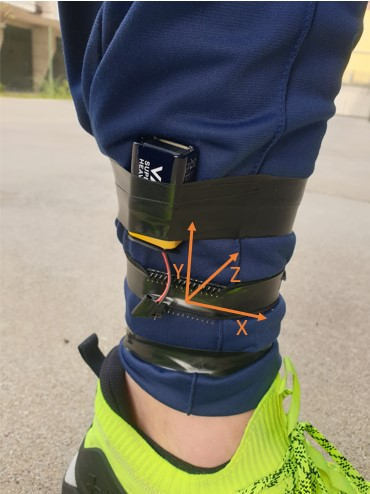
\includegraphics[width=0.4\linewidth]{./ImageFiles/arduino_su_gamba_frame.jpg}
	\caption{Arduino posizionato sulla gamba del soggetto con relativo sistema di riferimento.}
	\label{fig:arduino_su_gamba}
\end{figure}

\noindent
Per poter acquisire i dati con Arduino, è stato necessario sviluppare un firmware apposito che consentisse di inviare le misure utilizzando la tecnologia Bluetooth Low Energy (BLE), in cui l'Arduino viene utilizzato nel ruolo di \textit{peripheral} mentre l'applicazione assume il ruolo di \textit{central}. La board di Arduino espone un servizio con una caratteristica su cui vengono scritti i dati delle misure secondo il seguente formato: \\
\centerline{\texttt{"accx,accy,accz,gyrox,gyroy,gyroz,temp,hr,timestamp"}.}
Il central viene notificato ogni volta che il \textit{peripheral} aggiorna la caratteristica e, dopo averne letto il contenuto, salva le misure in un file .csv che contiene le seguenti colonne: \textit{accx}, \textit{accy}, \textit{accz}, \textit{gyrox}, \textit{gyroy}, \textit{gyroz}, \textit{temp}, \textit{hr} e \textit{timestamp}. Sull'applicazione è possibile visualizzare i dati ricevuti in tempo reale su un grafico (\Fig\ref{fig:schermata_acq}).
\begin{figure}[b!]
	\centering
	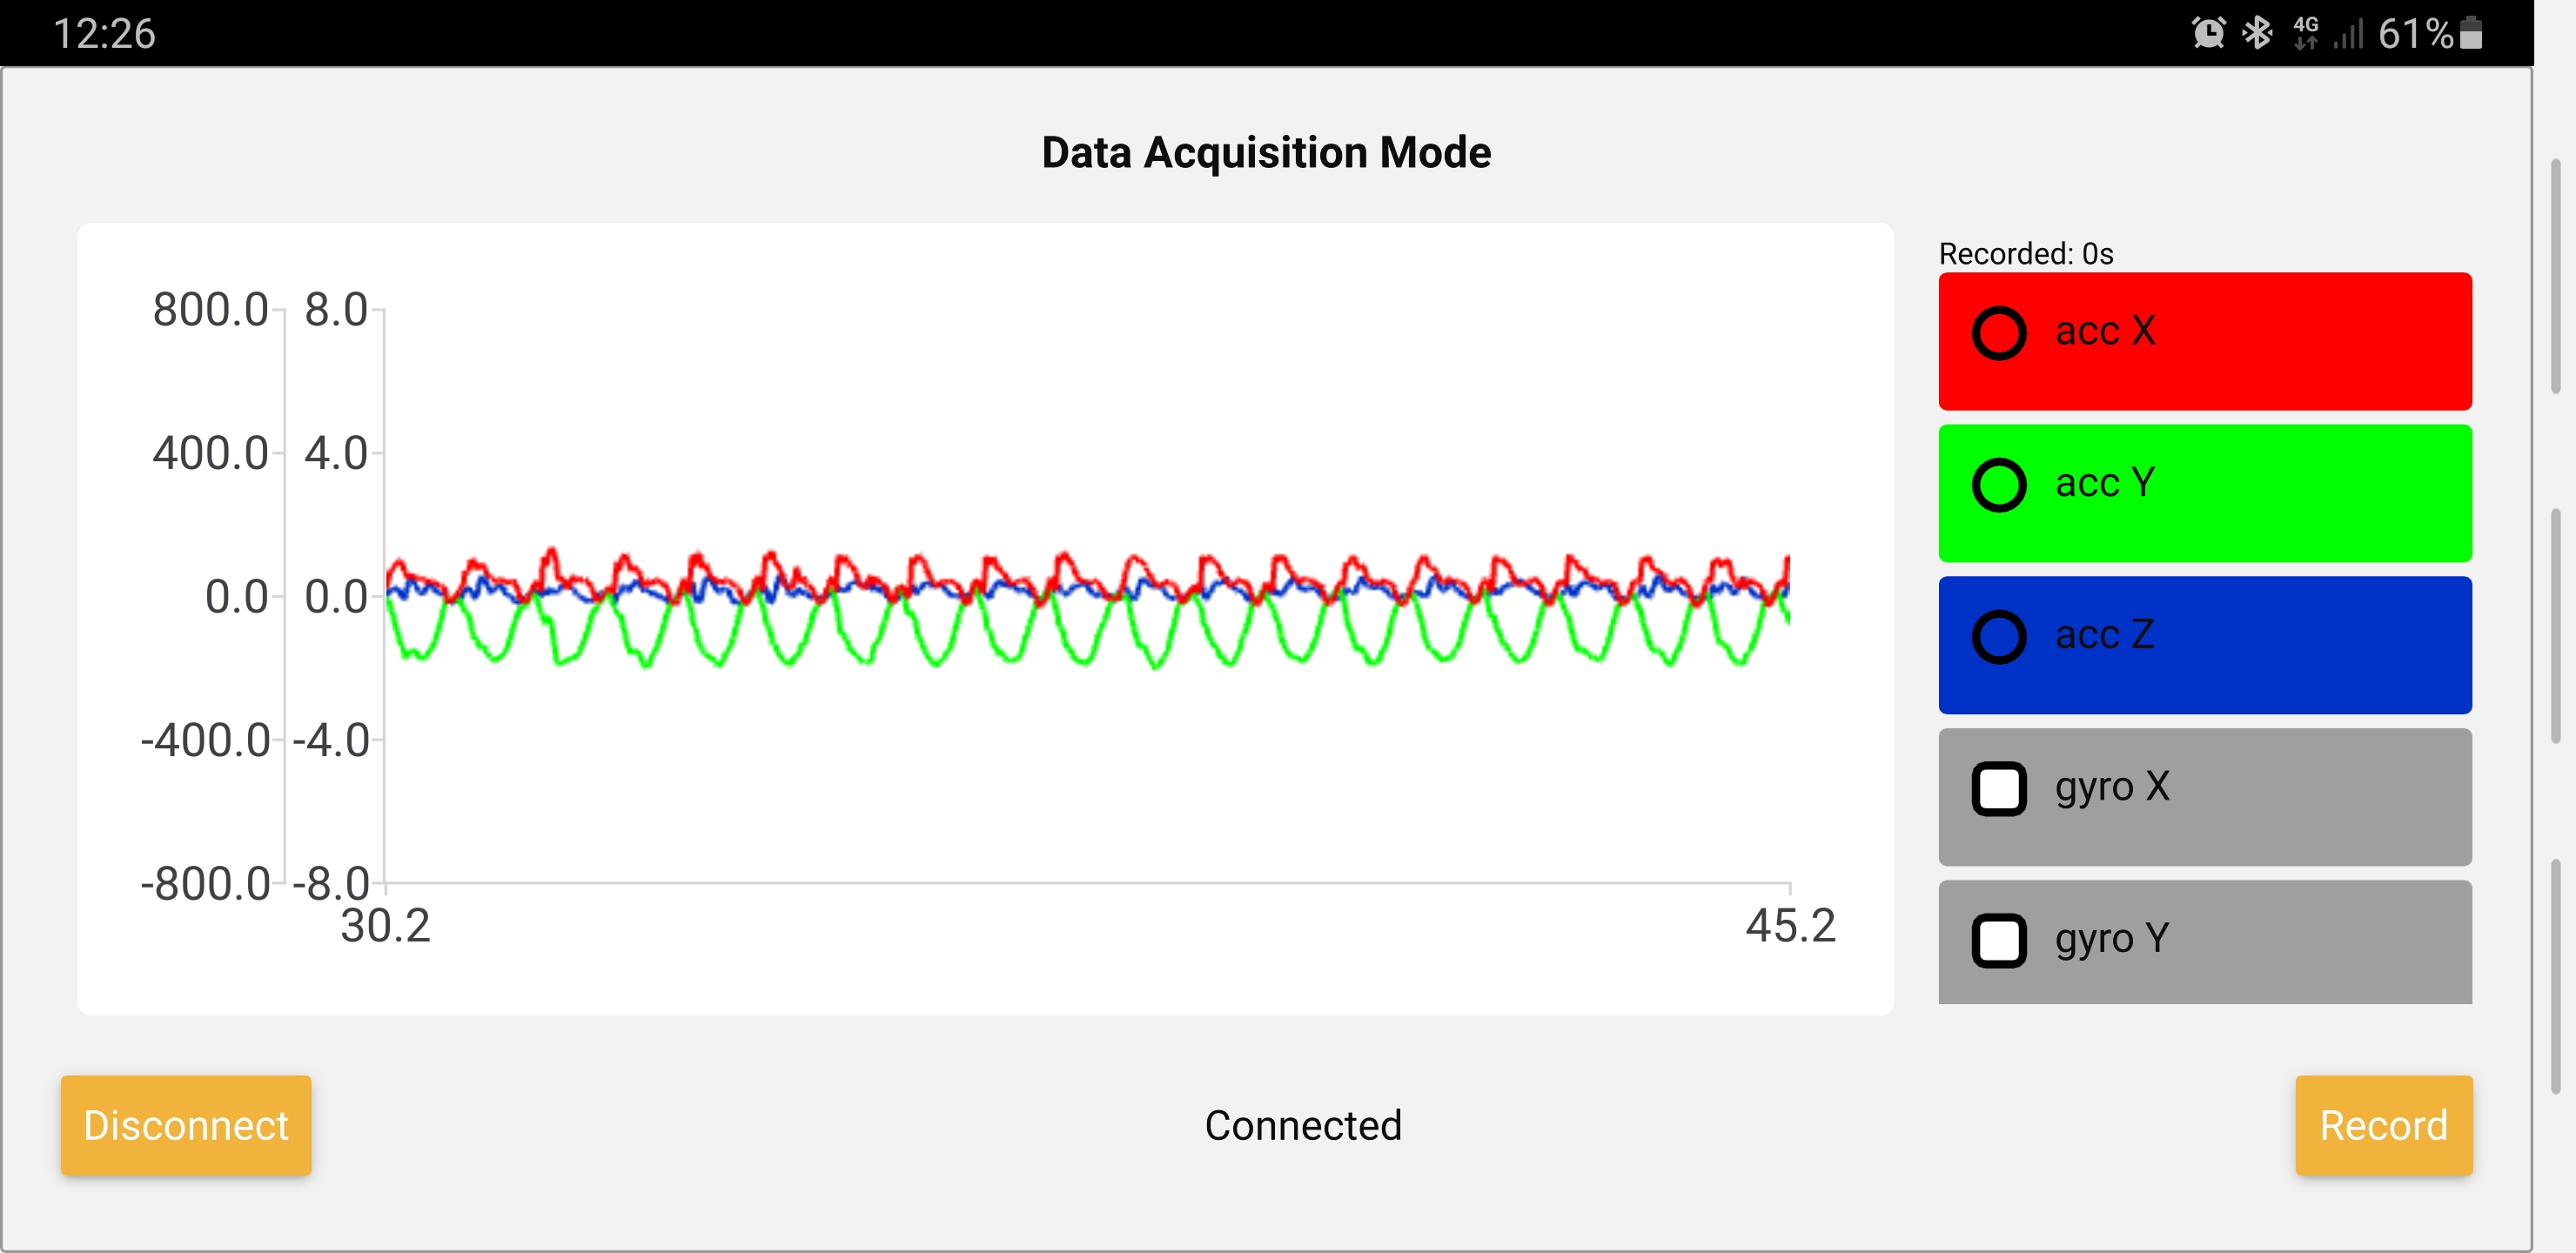
\includegraphics[width=0.49\linewidth]{./ImageFiles/acquisition_acc.jpg}
	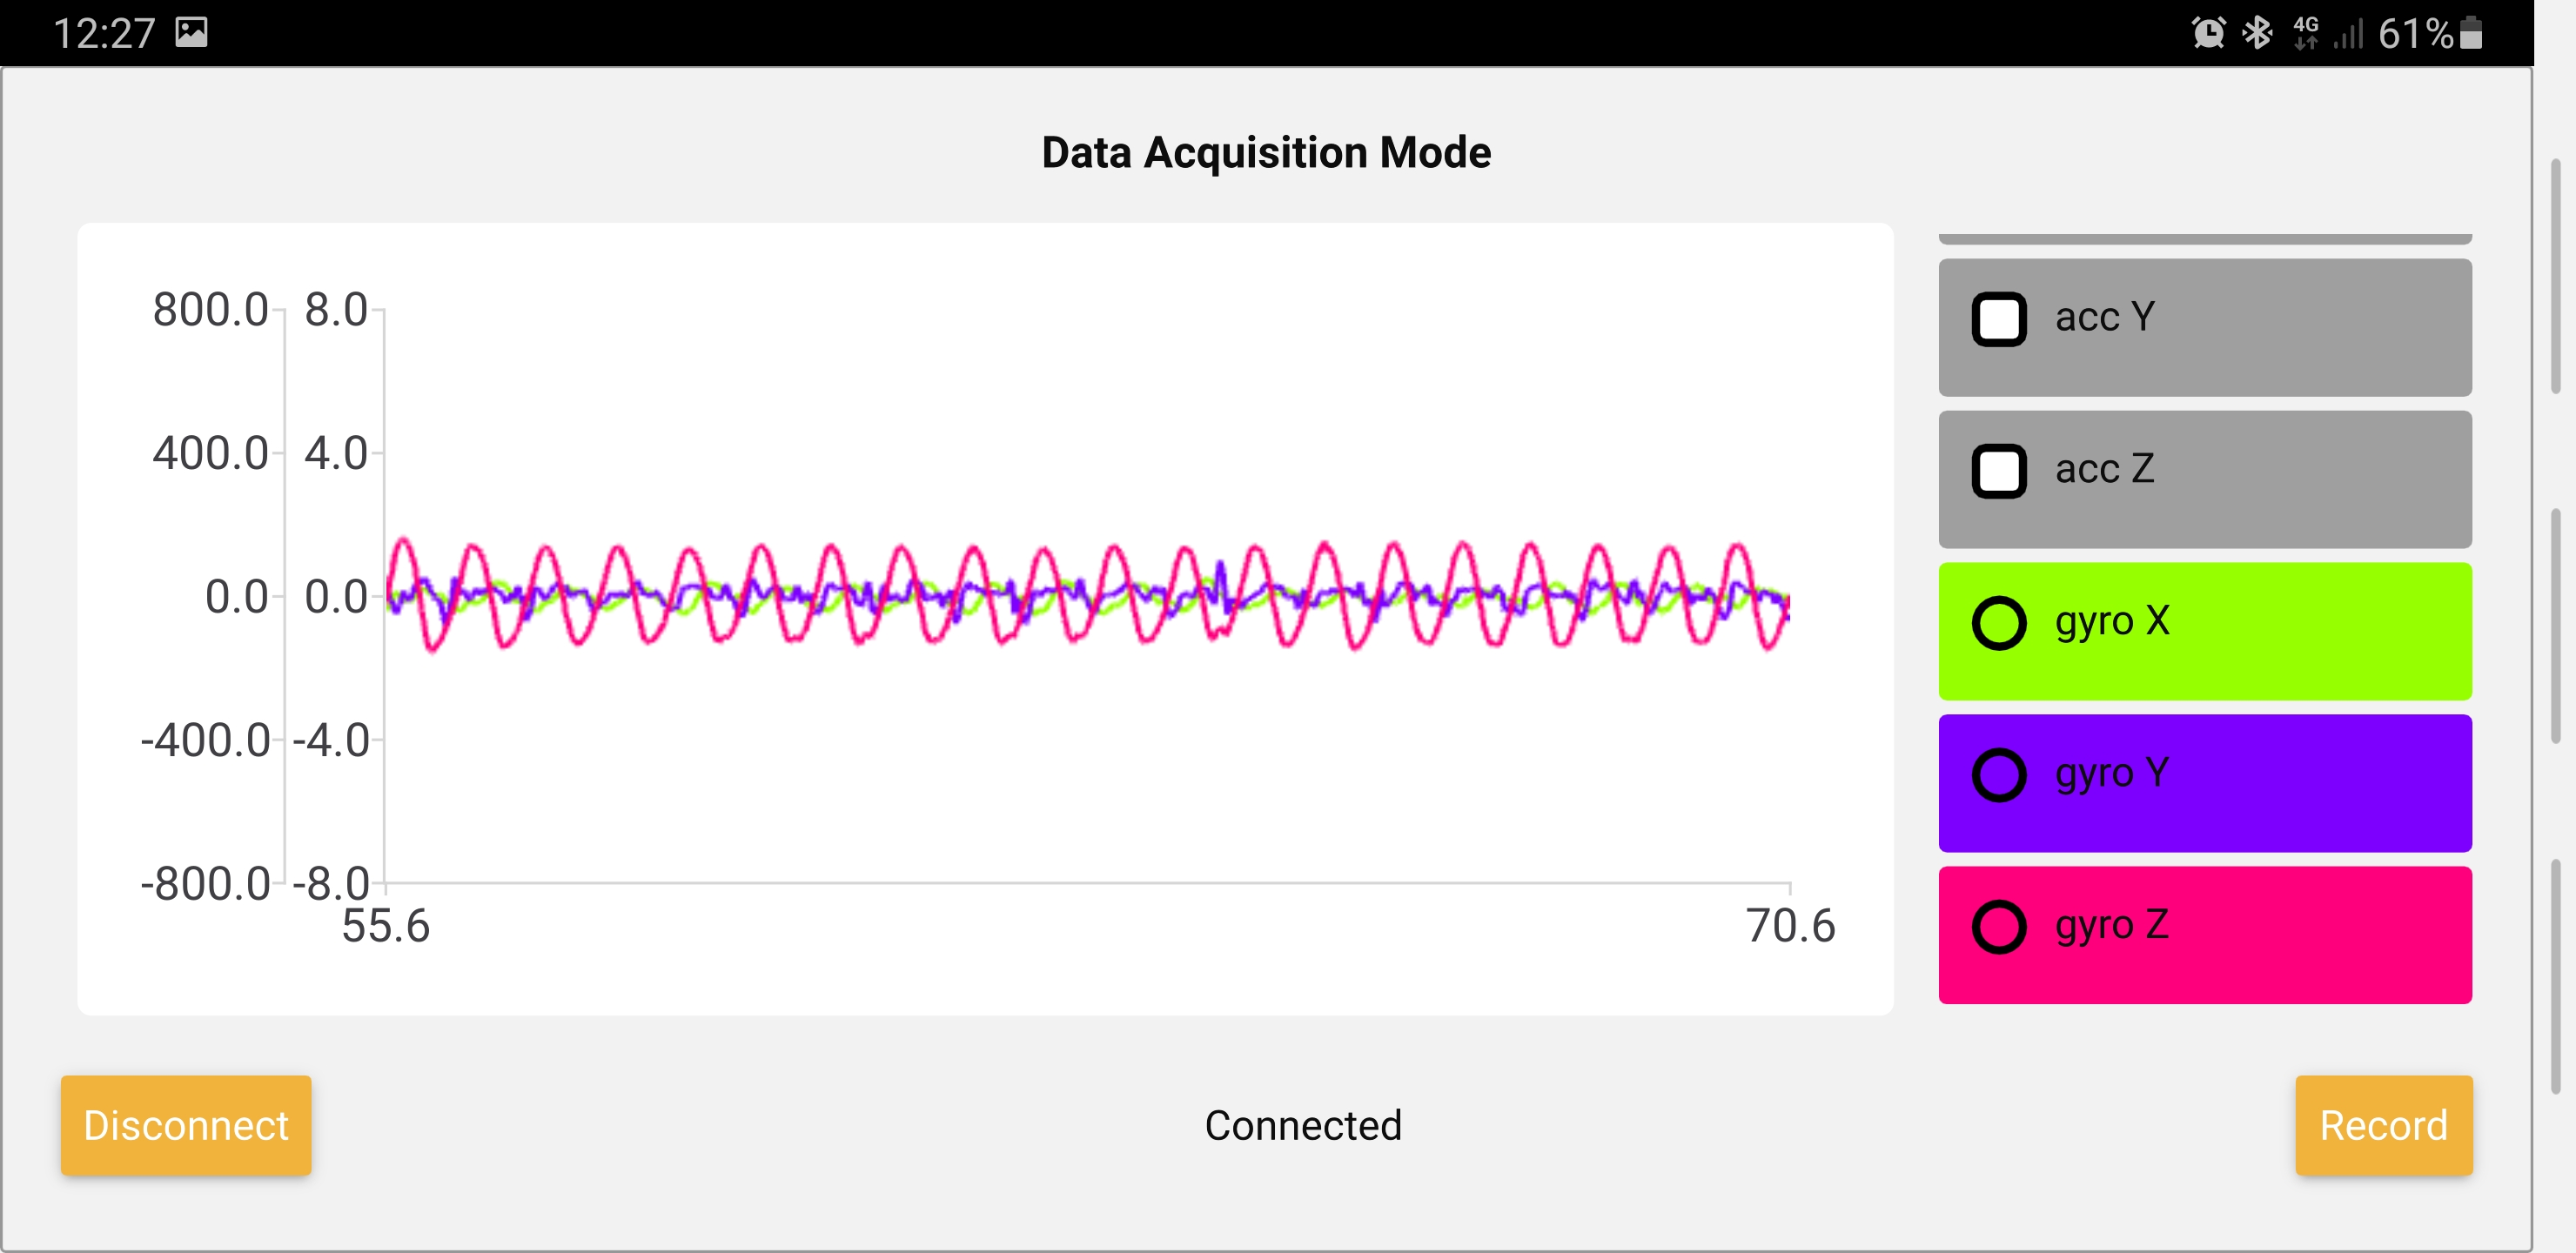
\includegraphics[width=0.49\linewidth]{./ImageFiles/acquisition_gyro.jpg}
	\caption{Schermata di acquisizione dati dell'applicazione: l'immagine a sinistra mostra i segnali dell'accelerometro mentre quella a destra mostra i segnali del giroscopio durante l'attività cyclette.}
	\label{fig:schermata_acq}
\end{figure}
Inizialmente, si è cercato di utilizzare una frequenza di campionamento dei dati pari a \SI{100}{\hertz}. Tuttavia, si è verificato che il flusso di dati non era sostenibile dal BLE. Tramite delle prove si è poi stabilito che una frequenza di campionamento dei dati sostenibile era di circa \SI{66}{\hertz} (un campione ogni \SI{15}{\milli\second}). Per assicurare una buona precisione nella frequenza di campionamento, si è scelto di utilizzare il meccanismo degli interrupt (Interrupt Service Routine), in cui una funzione di callback viene chiamata ogni \SI{15}{\milli\second}. Infatti, non è possibile utilizzare la funzione \textit{delay} poiché non garantisce intervalli regolari di acquisizione. Inoltre, ciò permette di realizzare un'applicazione \textit{pseudo} concorrente, in cui la funzione \textit{loop} principale si occupa dell'invio dei dati tramite BLE, mentre un'altra funzione, attivata da un interrupt, si occupa di acquisire i dati. Tuttavia, l'utilizzo degli interrupt non si è mostrato essere sufficiente a garantire una frequenza di campionamento accurata in quanto si è visto che il tempo necessario all'invio dei dati tramite BLE non è costante e ciò portava alla perdita di alcuni dati.
Per questo motivo, è stato introdotto un buffer circolare tramite la libreria \url{https://github.com/rlogiacco/CircularBuffer}. In questo modo, se la comunicazione subisce un ritardo non si ha perdita di dati. Di seguito è stato riportato un esempio dei dati dell'accelerometro e giroscopio ottenuti durante una camminata di un soggetto (\Fig\ref{fig:imu_data}).
\begin{figure}[tbh]
	\centering
	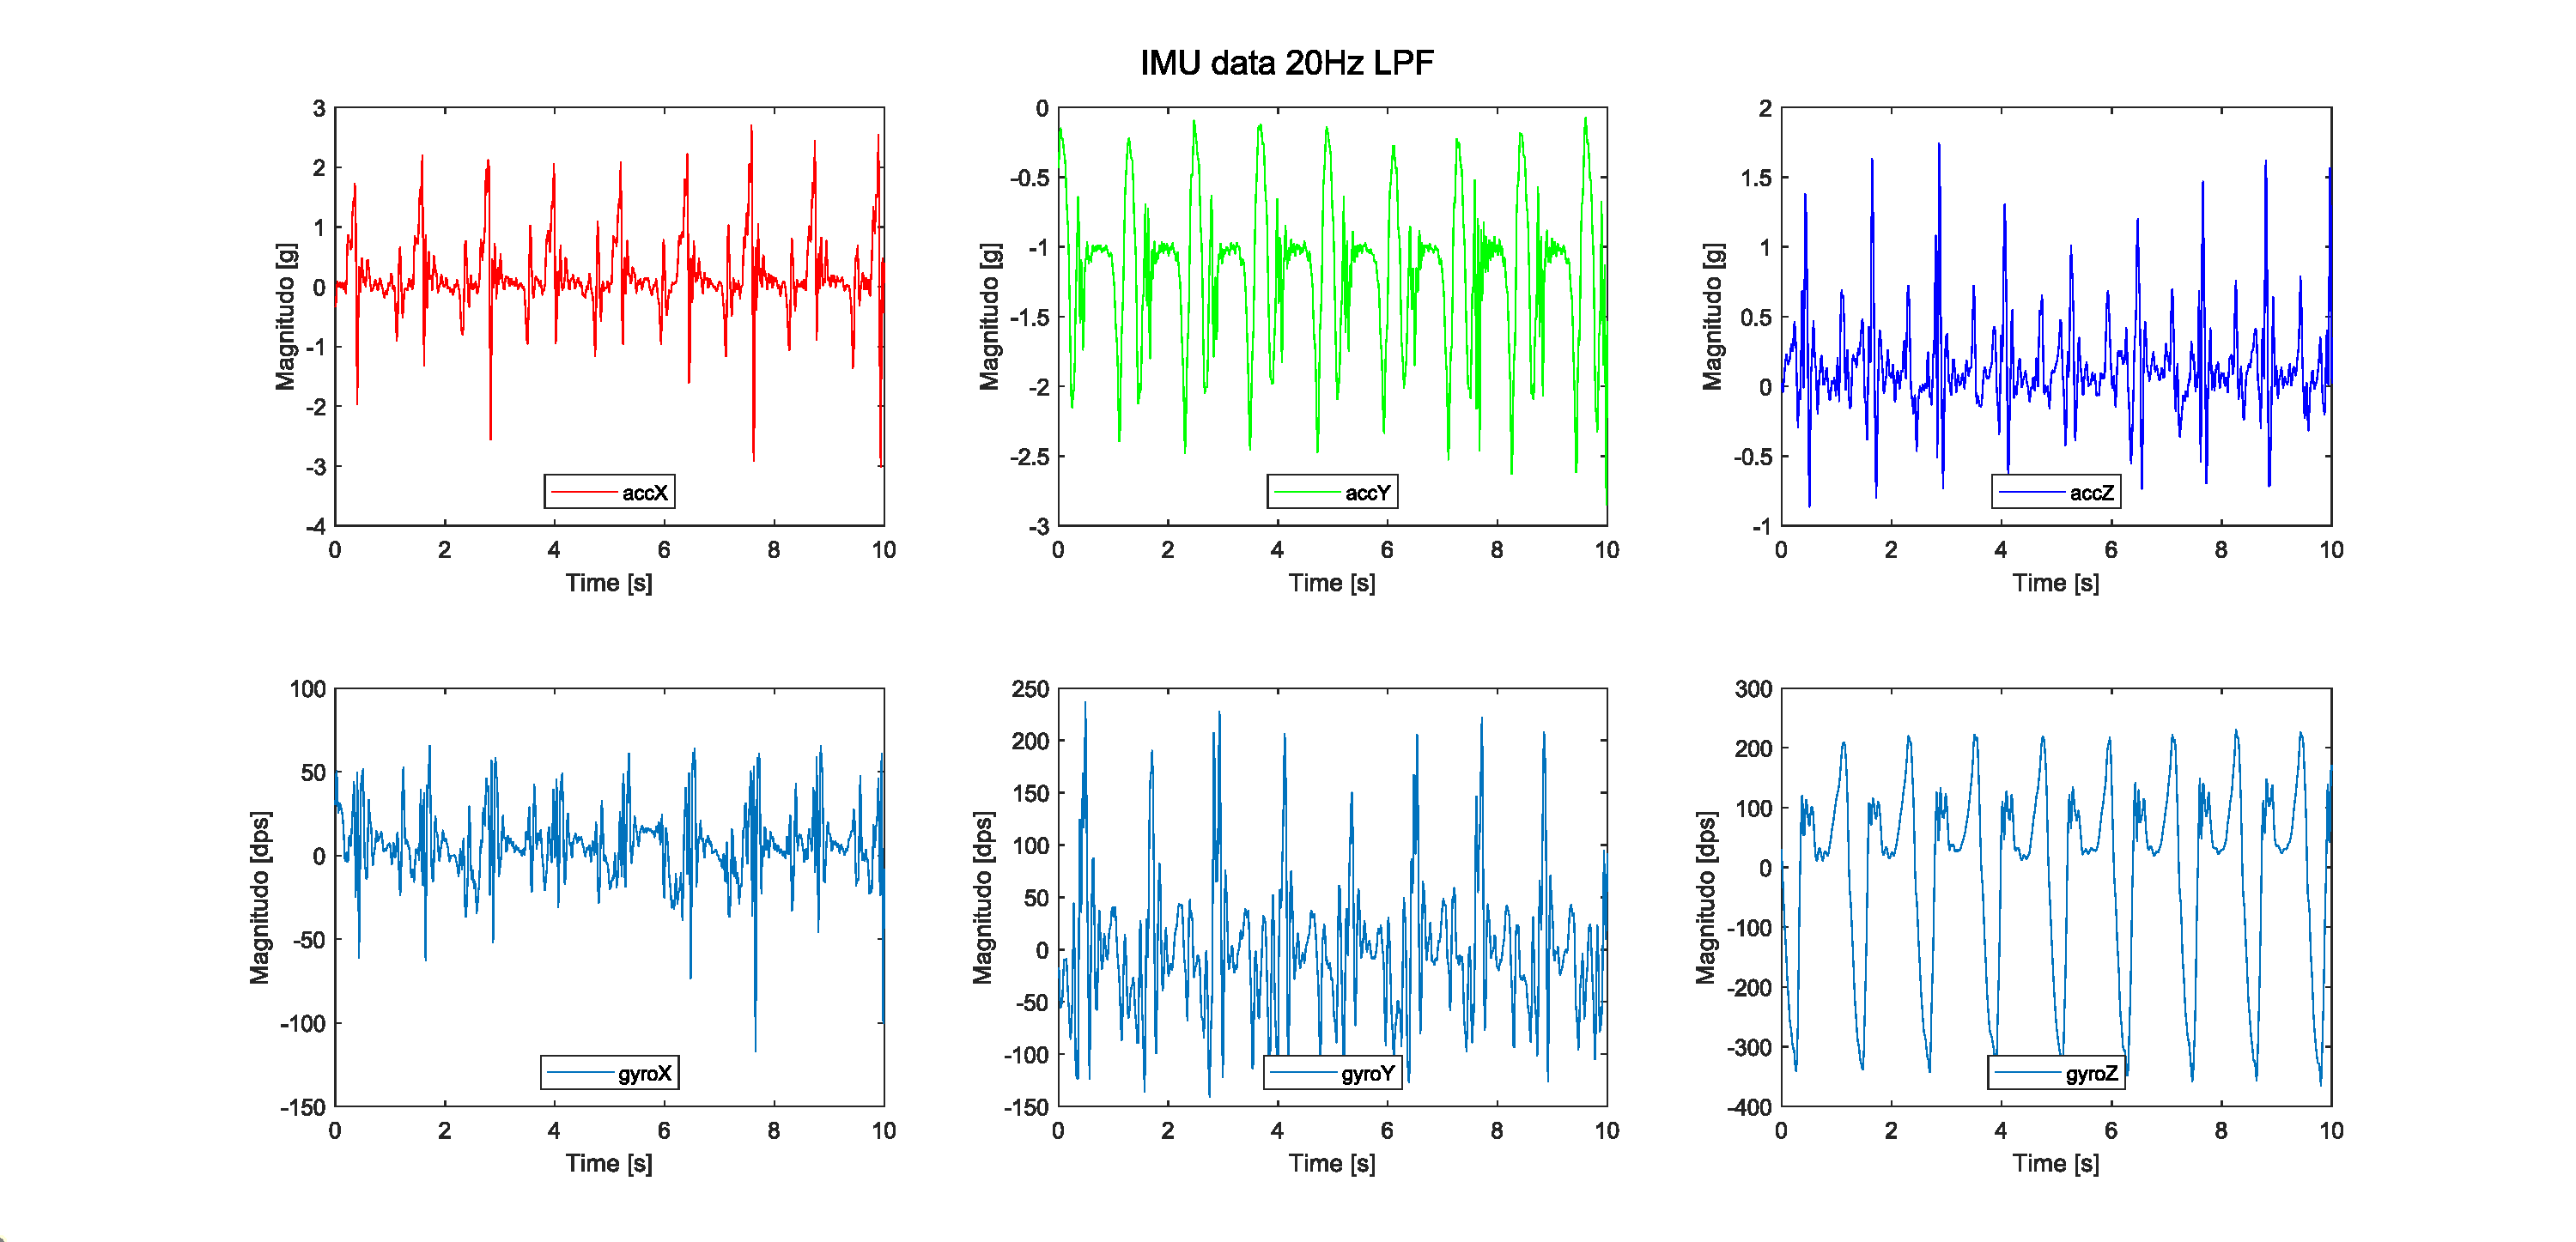
\includegraphics[width=1\linewidth]{./ImageFiles/IMU_data_example.pdf}
	\caption{Dati acquisiti dall'accelerometro e giroscopio durante una camminata. I dati sono campionati ogni \SI{15}{\milli\second} e sono stati filtrati con un filtro passa basso con frequenza di taglio di \SI{20}{\hertz}.}
	\label{fig:imu_data}
\end{figure}

\noindent
Nella figura \ref{fig:time_interval} è stato riportato un confronto tra gli intervalli di tempo tra due acquisizioni successive su una misura di \SI{76}{\second} eseguita su un soggetto durante una camminata con e senza buffer circolare. Nella figura \ref{fig:time_interval}a) è stato utilizzato il buffer circolare e il tempo medio risultante è di \SI{15.0057}{\milli\second} con una deviazione standard di \SI{0.4405}{\milli\second}. Senza buffer circolare (\Fig\ref{fig:time_interval}b)) è stata ottenuta una media di circa \SI{16.1630}{\milli\second} con una deviazione standard di \SI{6}{\milli\second}: infatti, è possibile vedere nell'immagine che si hanno molti più outlier. Quindi l'utilizzo del buffer rende più robusto il sistema in caso di eventuali rallentamenti nell'invio dei dati. Si tenga in considerazione che l'istante di tempo in cui si eseguiva l'acquisizione è stato misurato con la funzione \textit{millis()}, che ha errore di $\pm \SI{1}{\milli\second}$. 
\begin{figure}[tbh]
	\centering
	a)
	\begin{minipage}{.900\textwidth}
		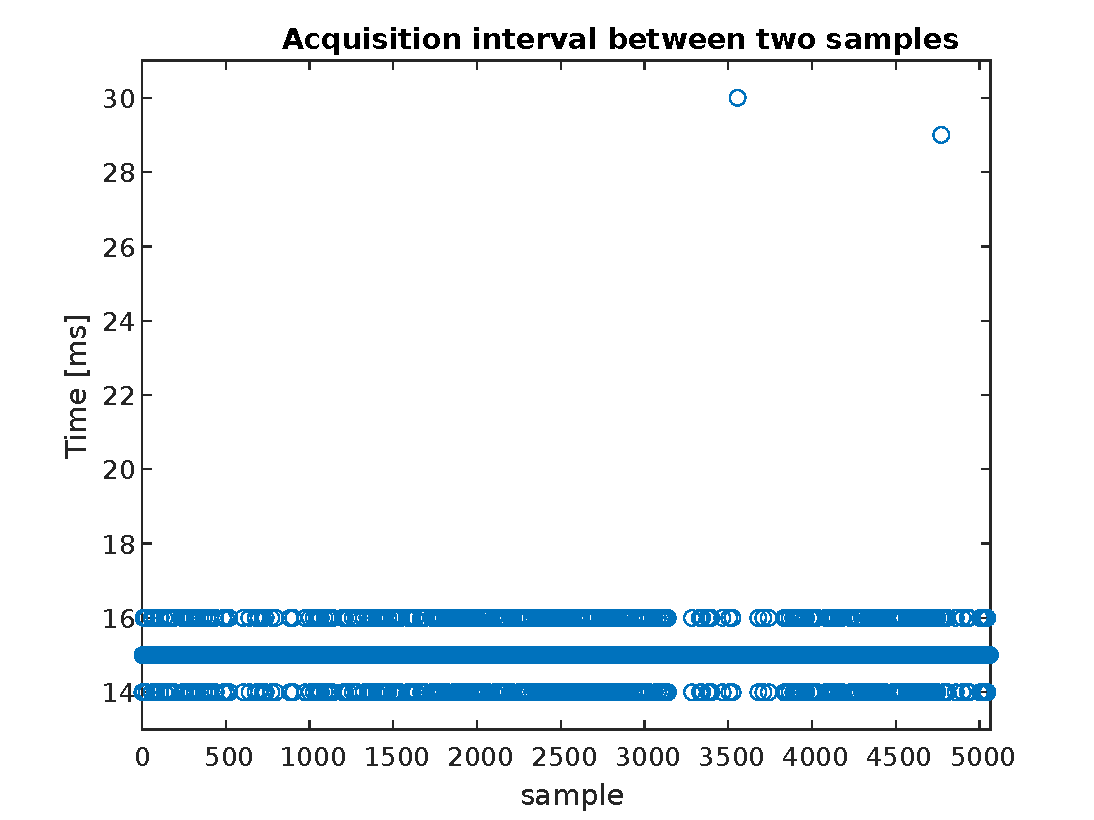
\includegraphics[width=0.8\linewidth]{./ImageFiles/interval_time.pdf}
	\end{minipage}
	\\b)
	\begin{minipage}{.900\textwidth}
		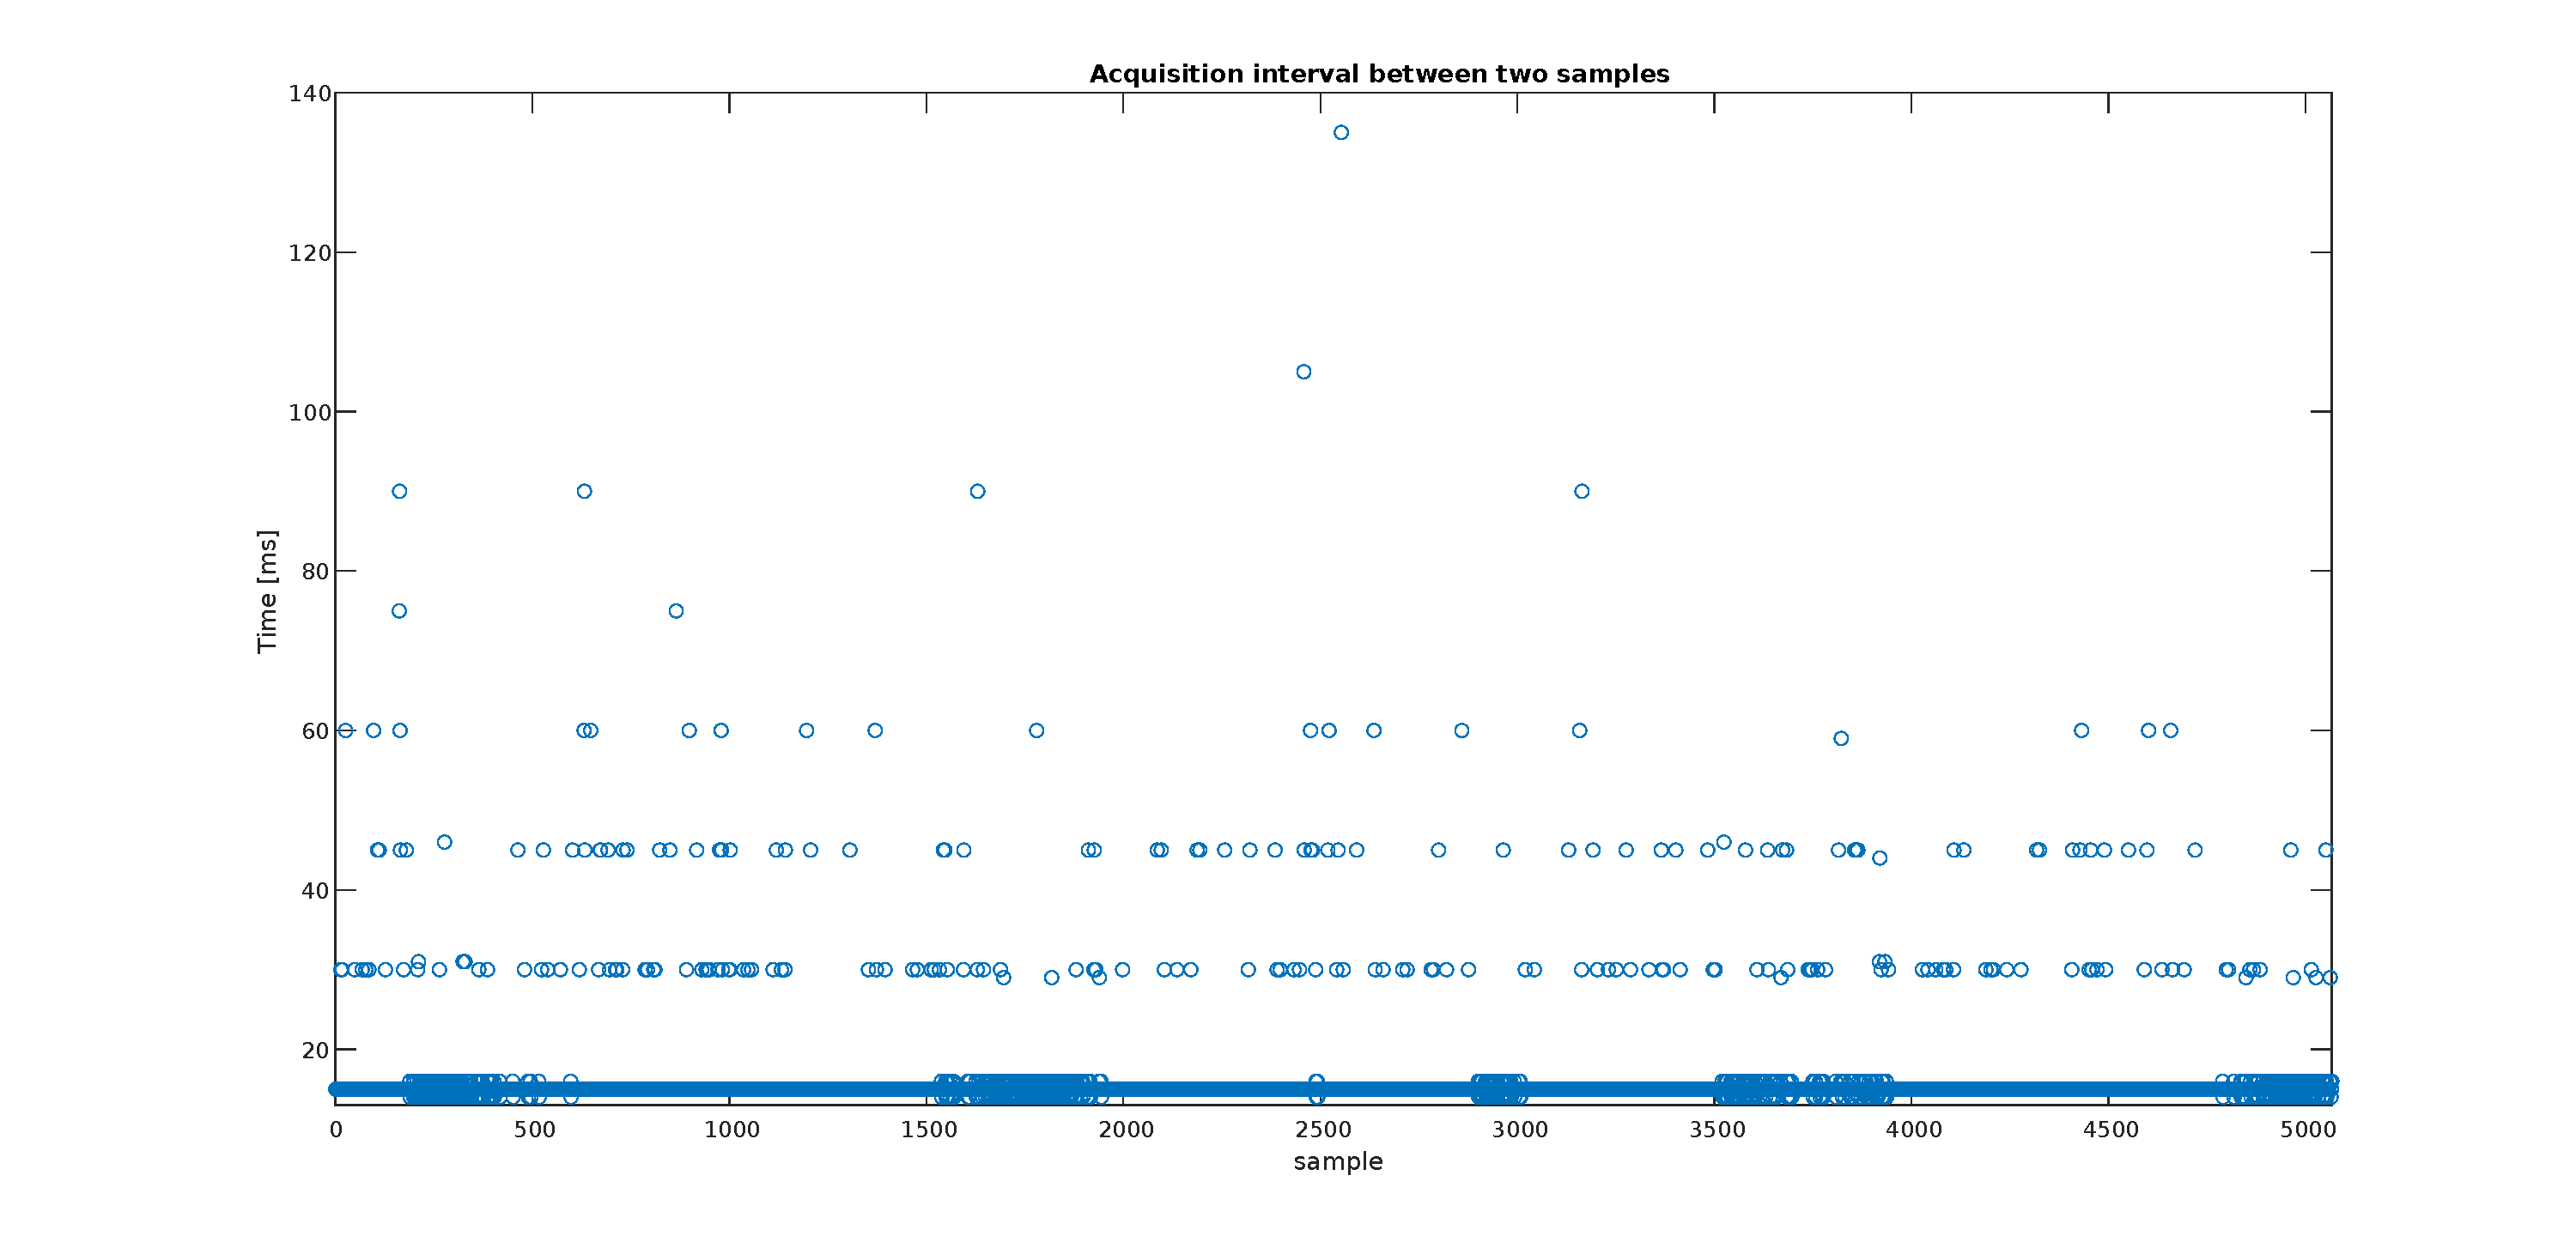
\includegraphics[width=\linewidth]{./ImageFiles/interval_time_2}
	\end{minipage}
	\caption{Tempo tra due campioni successivi su un'acquisizione di \SI{76}{\second}: a) con buffer circolare, b) senza buffer circolare.}
	\label{fig:time_interval}
\end{figure}

\clearpage

\section{Classificazione delle attività} \label{classifSect}
Nella figura \ref{fig:imu_data} è rappresentato un esempio di dati raccolti durante la camminata di un soggetto. Osservando i dati dell'accelerometro è possibile notare dei picchi che corrispondono ai movimenti dei passi del soggetto. In particolare, per come è stato posizionato l'Arduino (\Fig\ref{fig:imu_data}), è possibile notare il contributo della forza di gravità sull'asse y che causa un offset di circa 1g nelle misure e i picchi corrispondono a quando il piede entra in contatto con il terreno. Invece, per quanto riguarda le misure del giroscopio, è interessante notare lungo l'asse z il movimento di rotazione del piede attorno alla caviglia durante la camminata. 

Per realizzare la classificazione dei dati acquisiti dai sensori di Arduino e poi per visualizzarne la previsione sull'applicazione è stato sviluppato un ulteriore firmware al cui interno sono stati utilizzati tre thread differenti, analizzati più in dettaglio nella sezione \ref{arduinoSect}, che si occupano di ricavare i dati dalla IMU, effettuare la predizione ed inviare il risultato tramite BLE all'applicazione. In generale, il funzionamento del firmware prevede che inizialmente venga riempito un buffer circolare con i dati provenienti dai sensori. Successivamente, il buffer viene trasformato in un elenco di features tramite un DSP. Le features raccolte vengono poi passate al classificatore, realizzato grazie al framework Edge Impulse, che si occupa della classificazione. Infine, il risultato della classificazione viene trasmesso tramite BLE all'applicazione che mostra a video l'immagine relativa all'attività fisica identificata. Le schermate che possono essere visualizzate sull'applicazione si distinguono in base all'attività fisica rilevata come mostrato nella figura \ref{fig:attivitafisica}. Nei momenti subito dopo la connessione del dispositivo al BLE oppure nei momenti in cui non si riesce a classificare l'attività in corso sull'applicazione viene visualizzata la scritta \textit{"Unknown"}, che indica che il sistema non è in grado di riconosce l'attività.
\begin{figure}[tbh]
	\centering
	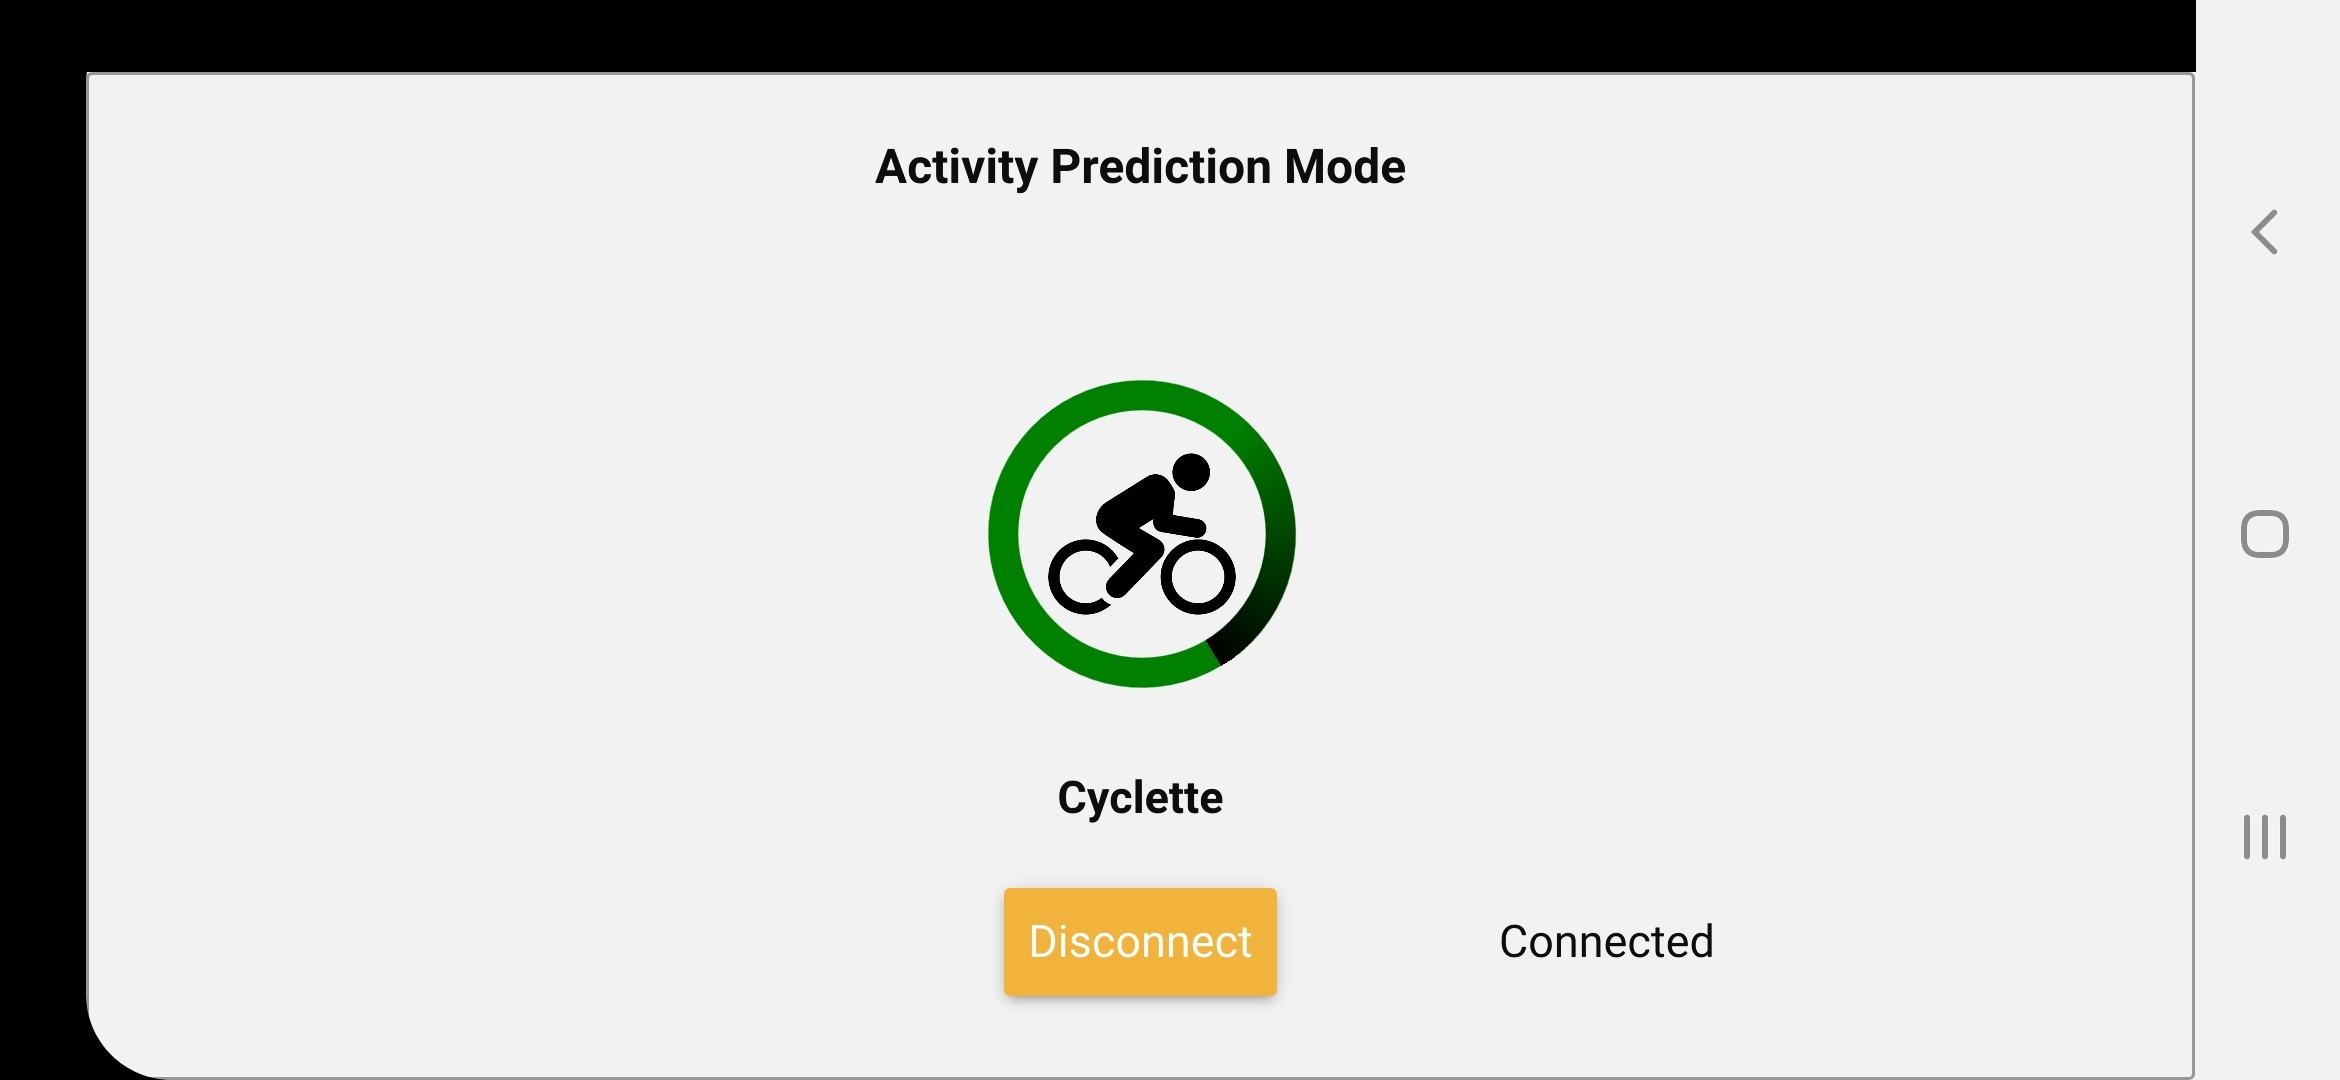
\includegraphics[width=0.4\linewidth]{./ImageFiles/cyclette}
	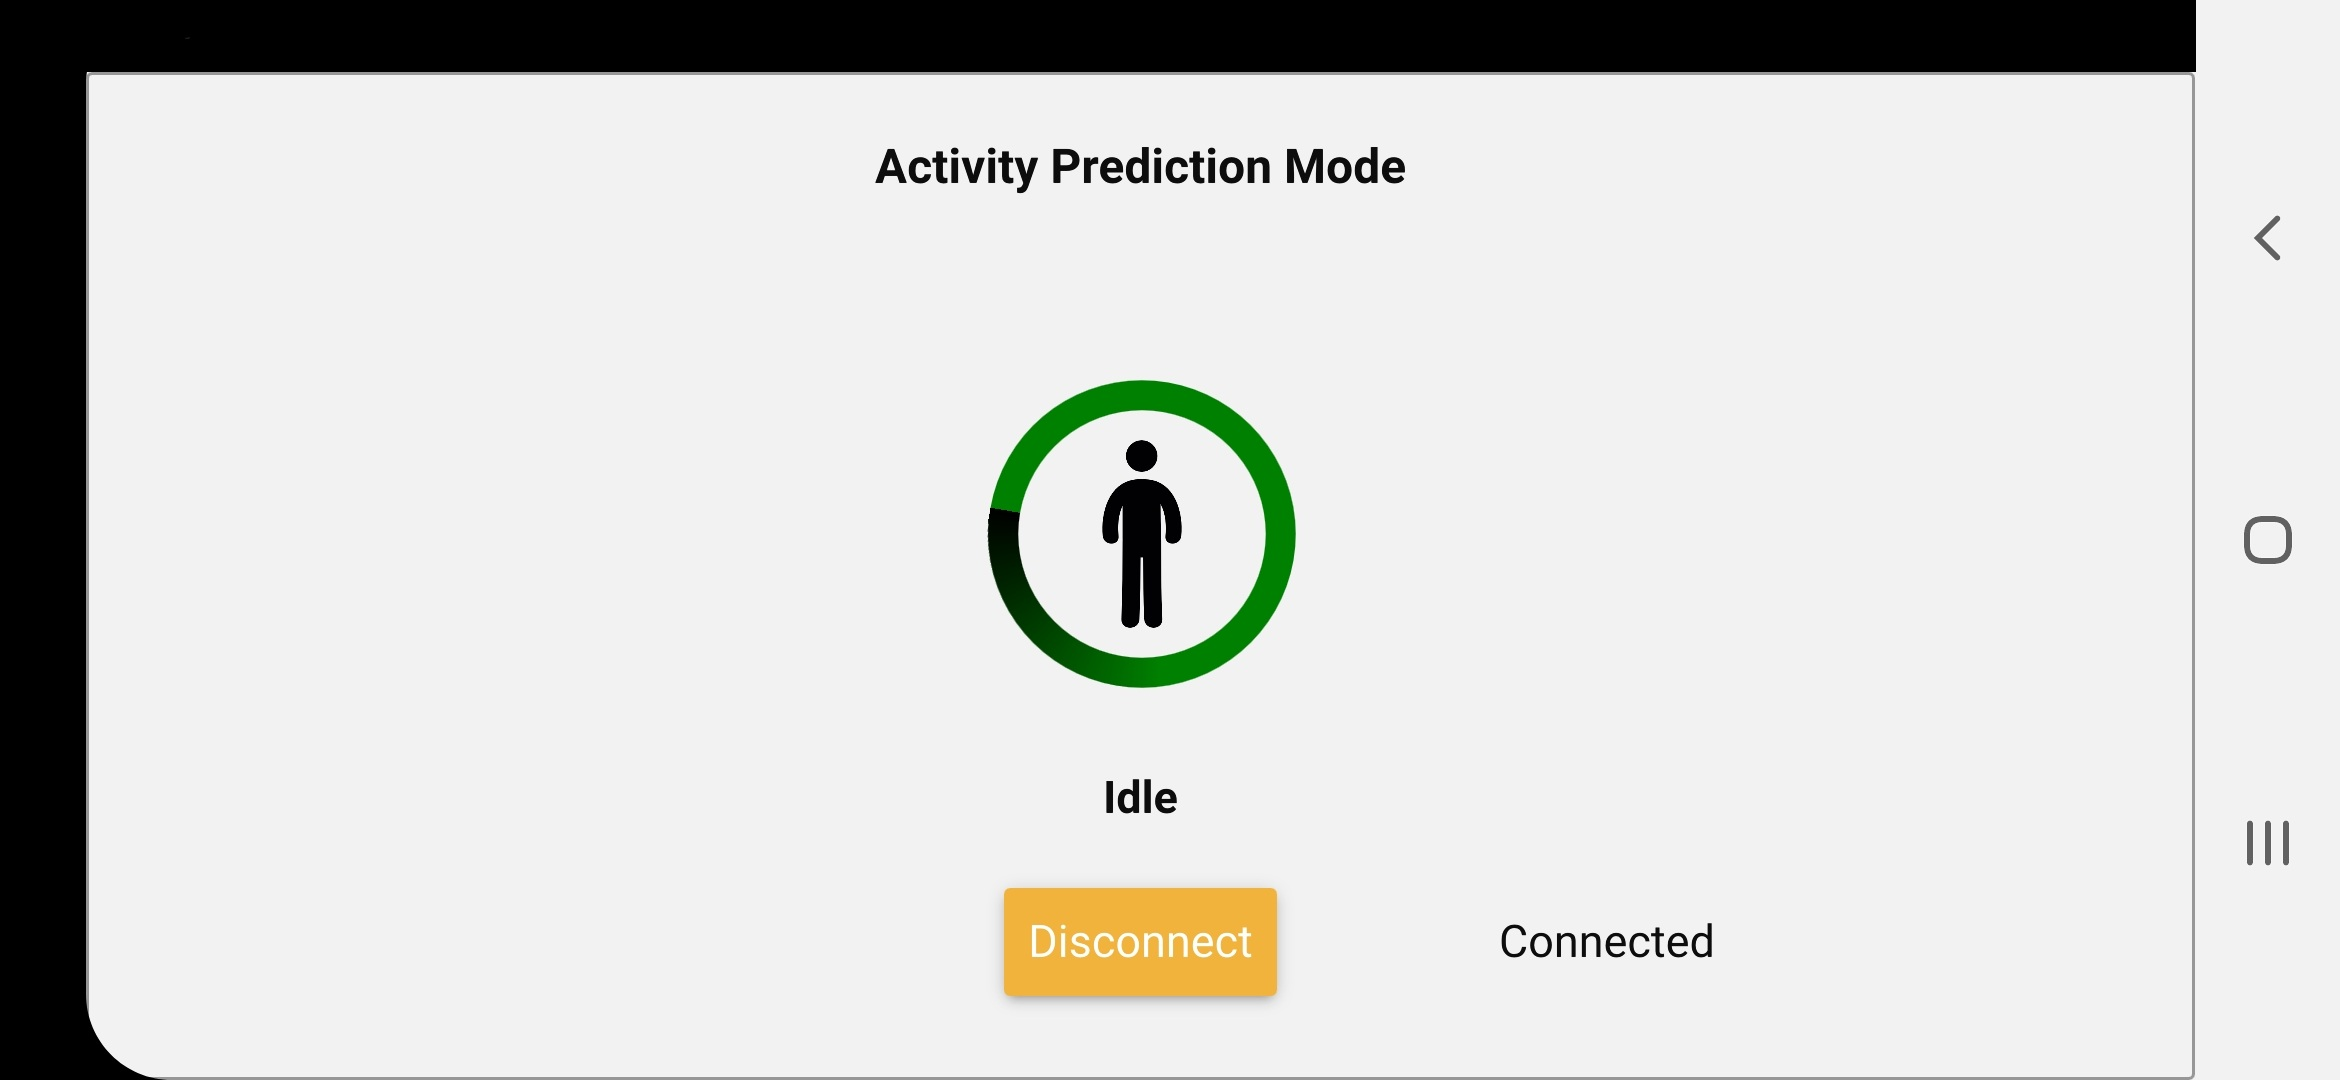
\includegraphics[width=0.4\linewidth]{./ImageFiles/idle}
	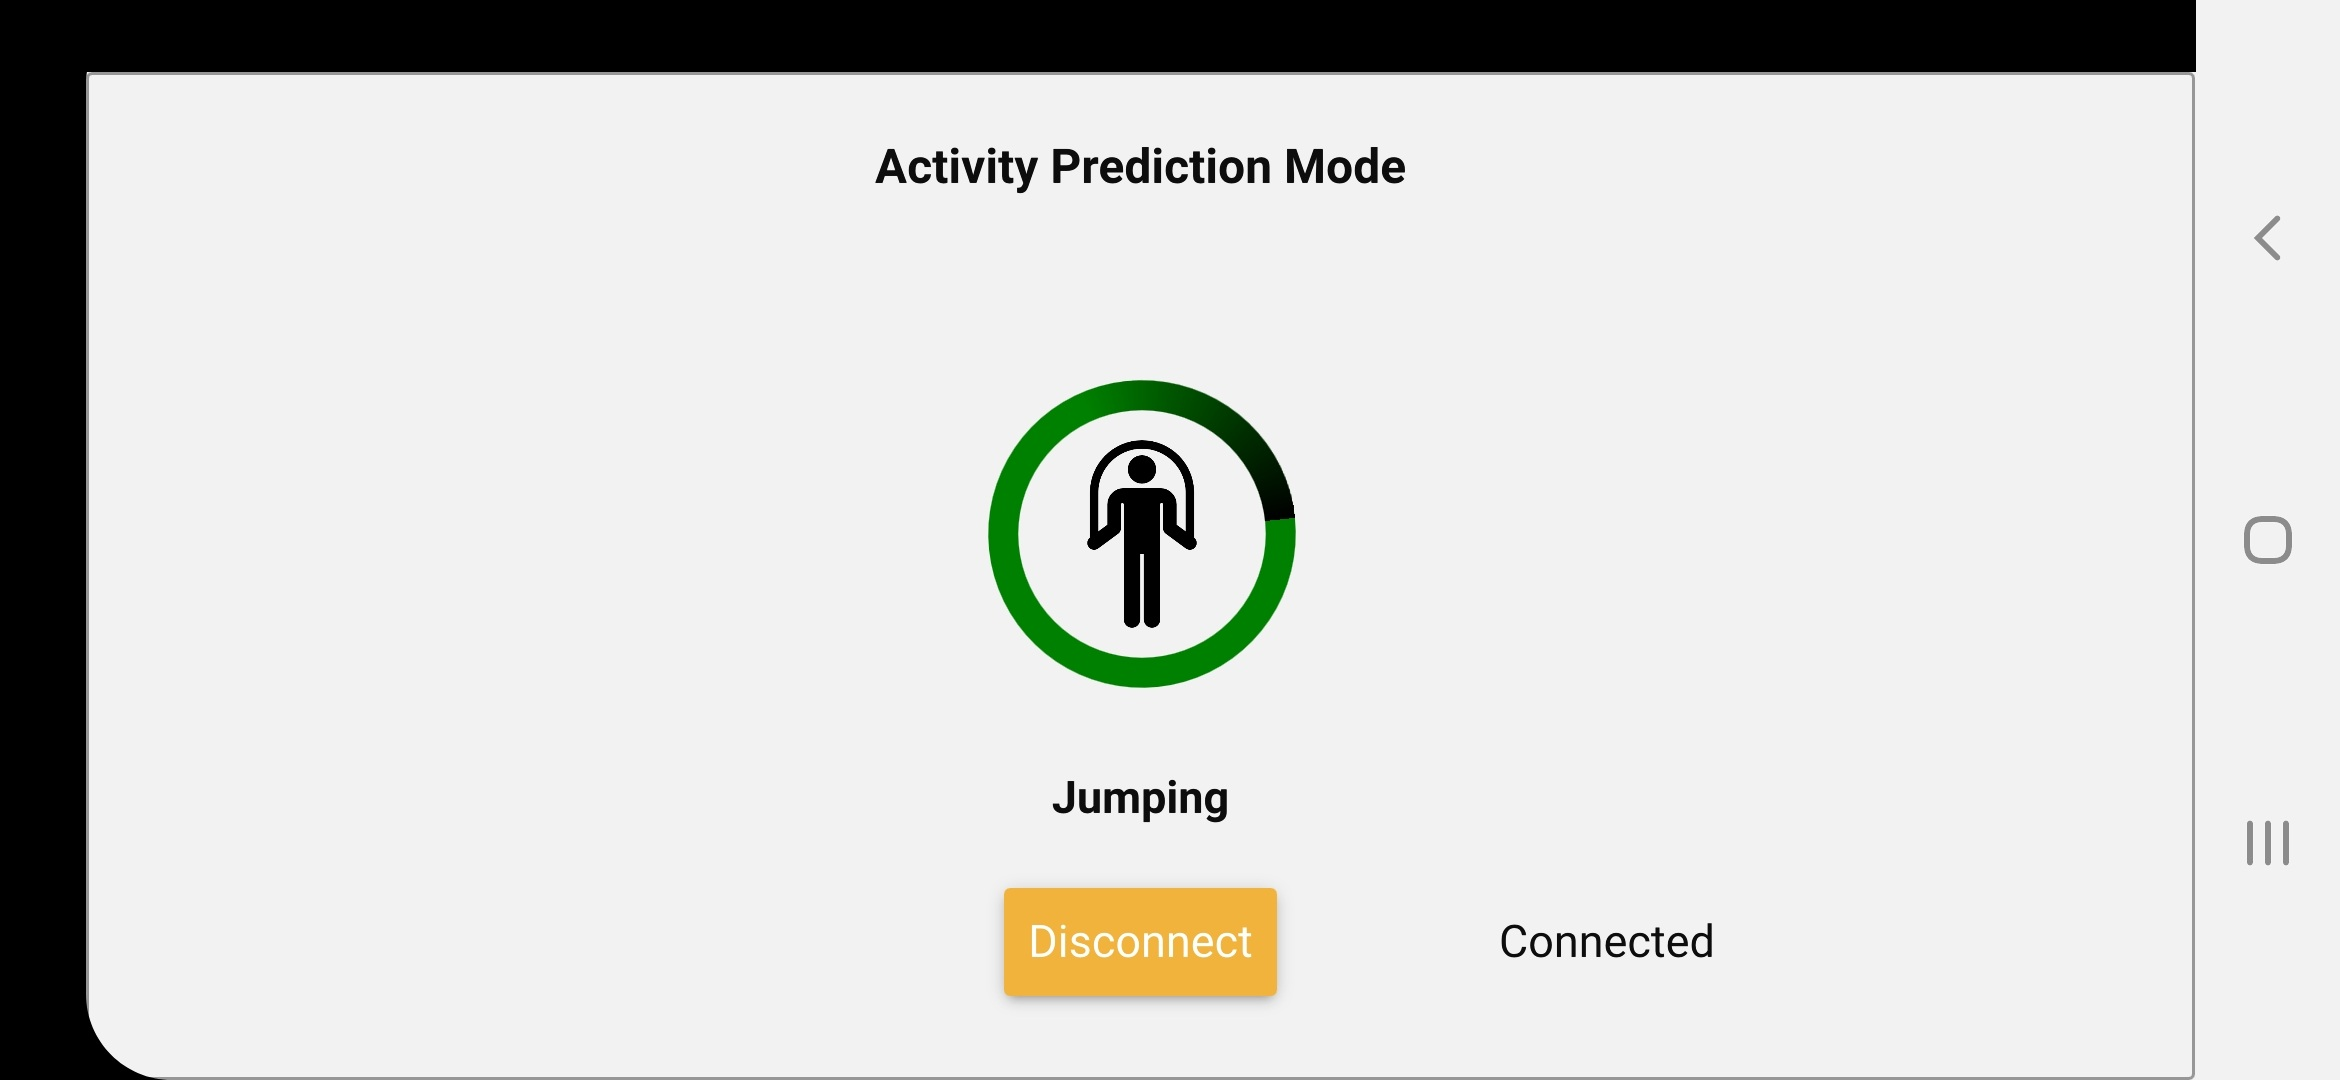
\includegraphics[width=0.4\linewidth]{./ImageFiles/jumping}
	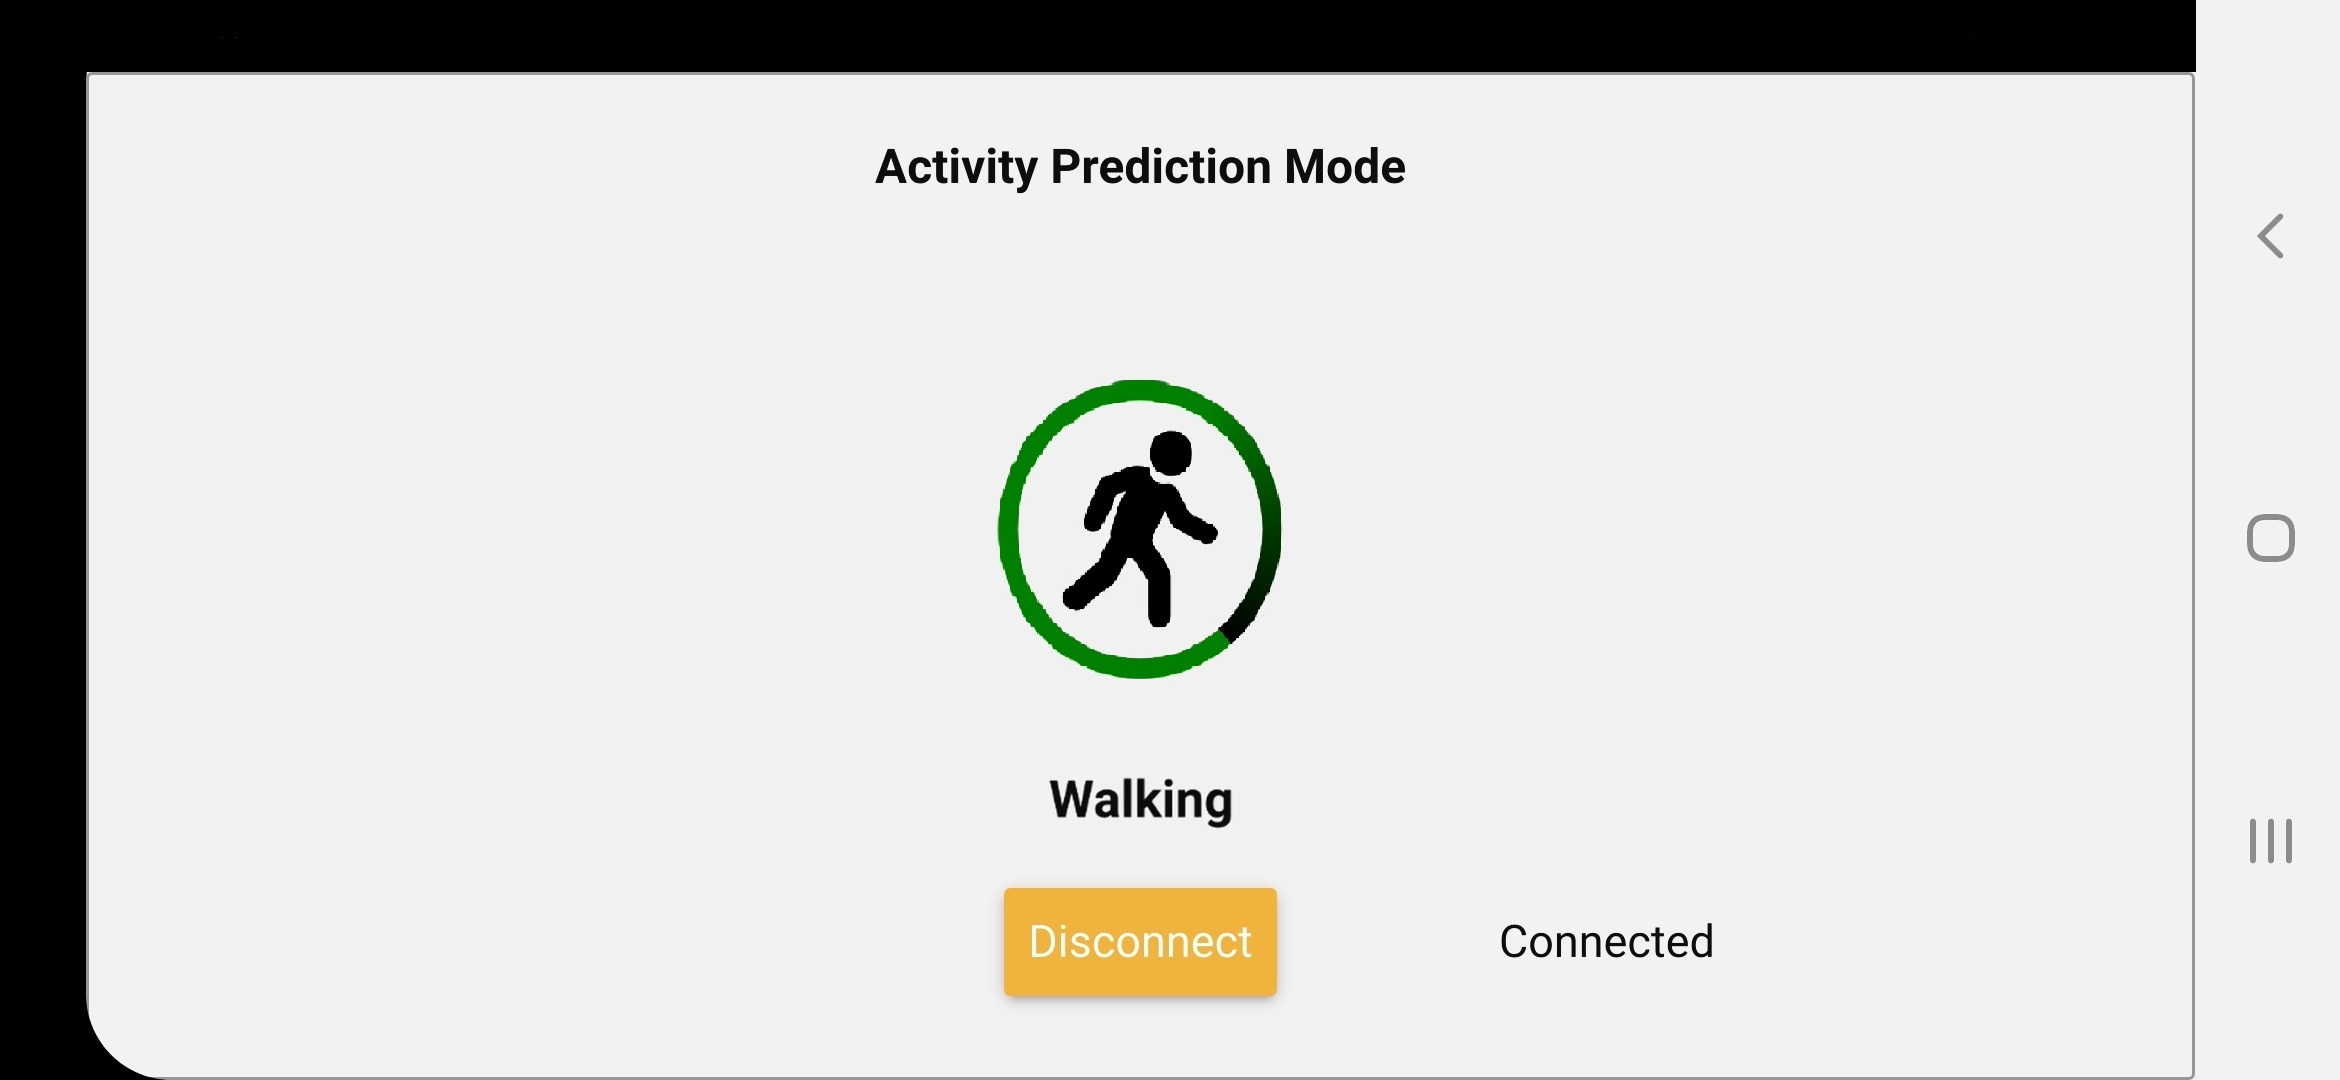
\includegraphics[width=0.4\linewidth]{./ImageFiles/walking}
	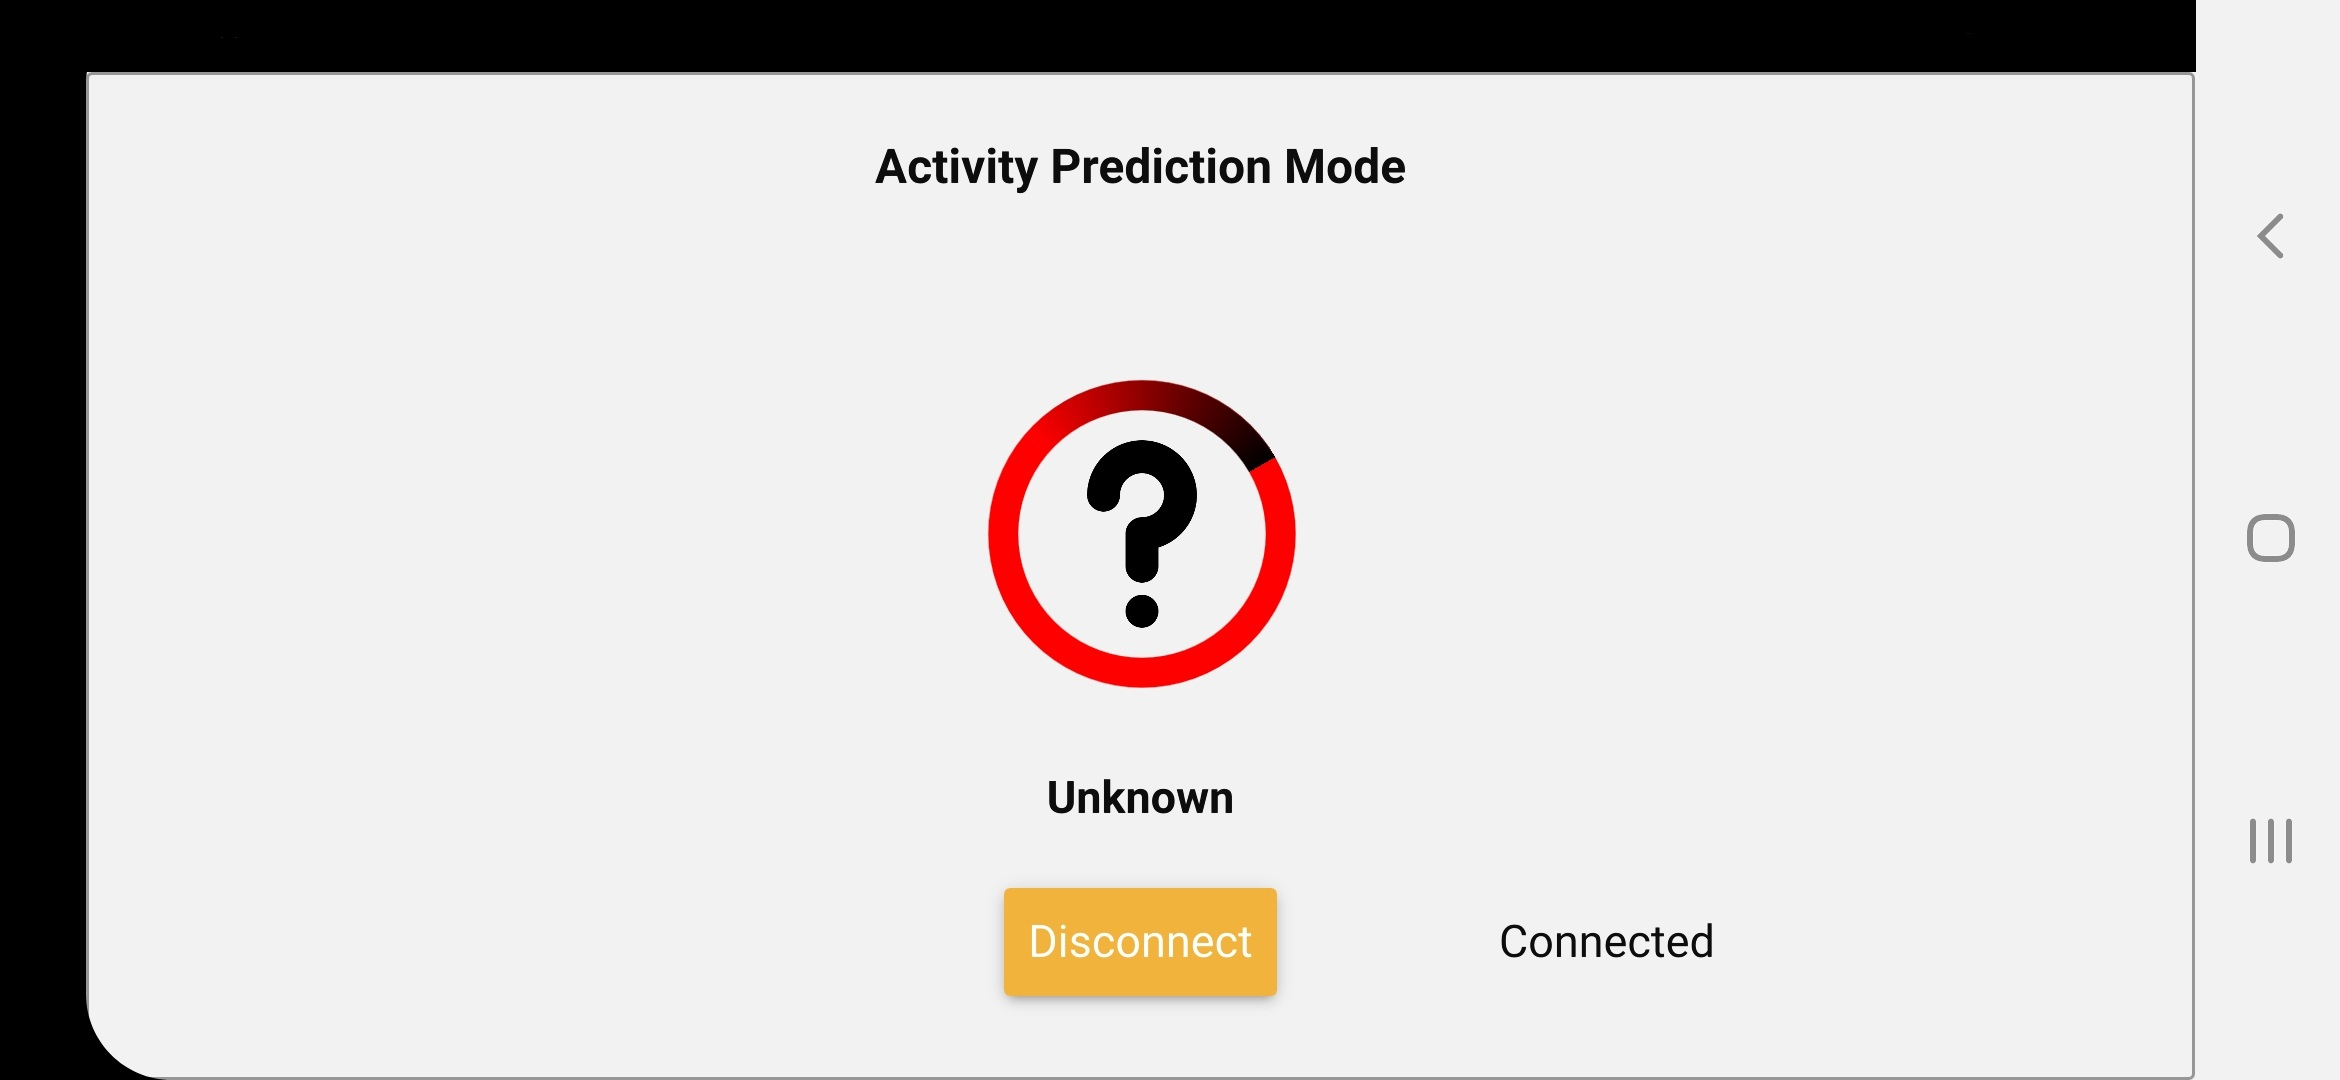
\includegraphics[width=0.4\linewidth]{./ImageFiles/unknown}
	\caption{Schermate per le possibili attività: cyclette, fermo, salto della corda, camminata e attività non riconosciuta.}
	\label{fig:attivitafisica}
\end{figure}

\subsection{Edge Impulse}
Edge Impulse è una piattaforma online per lo sviluppo di algoritmi di machine learning per \textit{edge devices}. Tramite Edge Impulse è possibile creare un modello da poter caricare sul dispositivo finale seguendo quattro semplici passi: acquisizione dei dati, design del modello, test del modello e deploy del modello. 

Per prima cosa sono stati acquisiti i dati delle quattro categorie di attività fisica da classificare (idle, walking, jumping e cycling). Per raccogliere i dati, è stato utilizzato il firmware precedentemente descritto, misurando attività per circa \SI{70}{\second}. Essendo un modello di \textit{machine learning}, maggiore è il numero dei dati, maggiore è la qualità del modello stimato. I dati acquisiti sono quindi stati caricati sulla piattaforma Edge Impulse dove sono stati divisi in \textit{training set} e \textit{test set} (\Fig\ref{fig:acquisizione_dati}). Edge Impulse suggerisce di dividere i dati di train e di test con una percentuale rispettivamente di 80\% e 20\%.
\begin{figure}[h!]
	\centering
	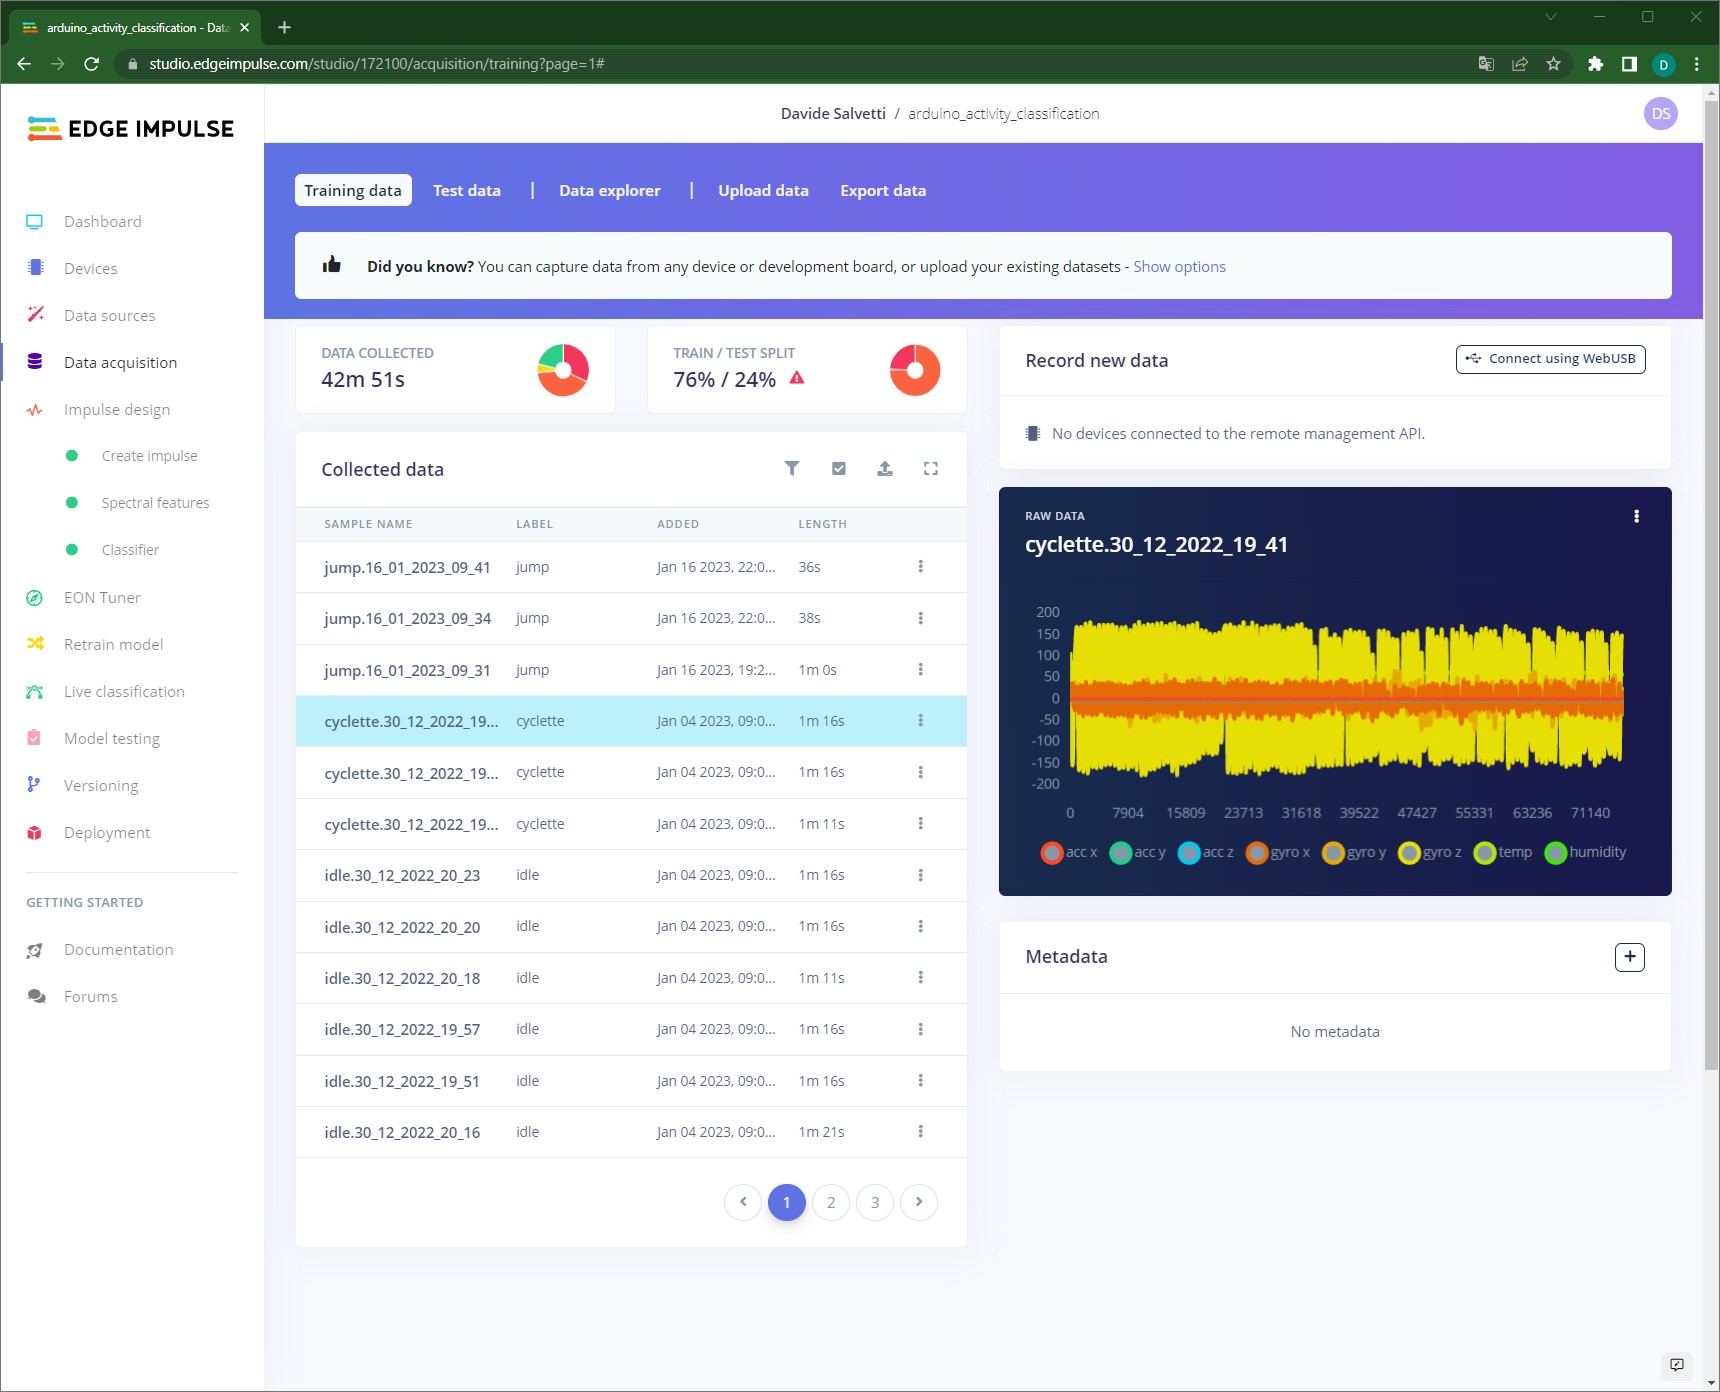
\includegraphics[width=0.5\linewidth]{./ImageFiles/data_acquisition.jpg}
	\caption{Pagina di Edge Impulse per l'inserimento di nuovi campioni.}
	\label{fig:acquisizione_dati}
\end{figure}

Successivamente, è stato creato un \textit{impulse}: questa fase prevede la selezione della larghezza della finestra dei dati che vengono poi processati, di un blocco di processamento dei dati e di un blocco di learning (figura \ref{fig:creazione_impulse}).
\begin{figure}[b!]
	\centering
	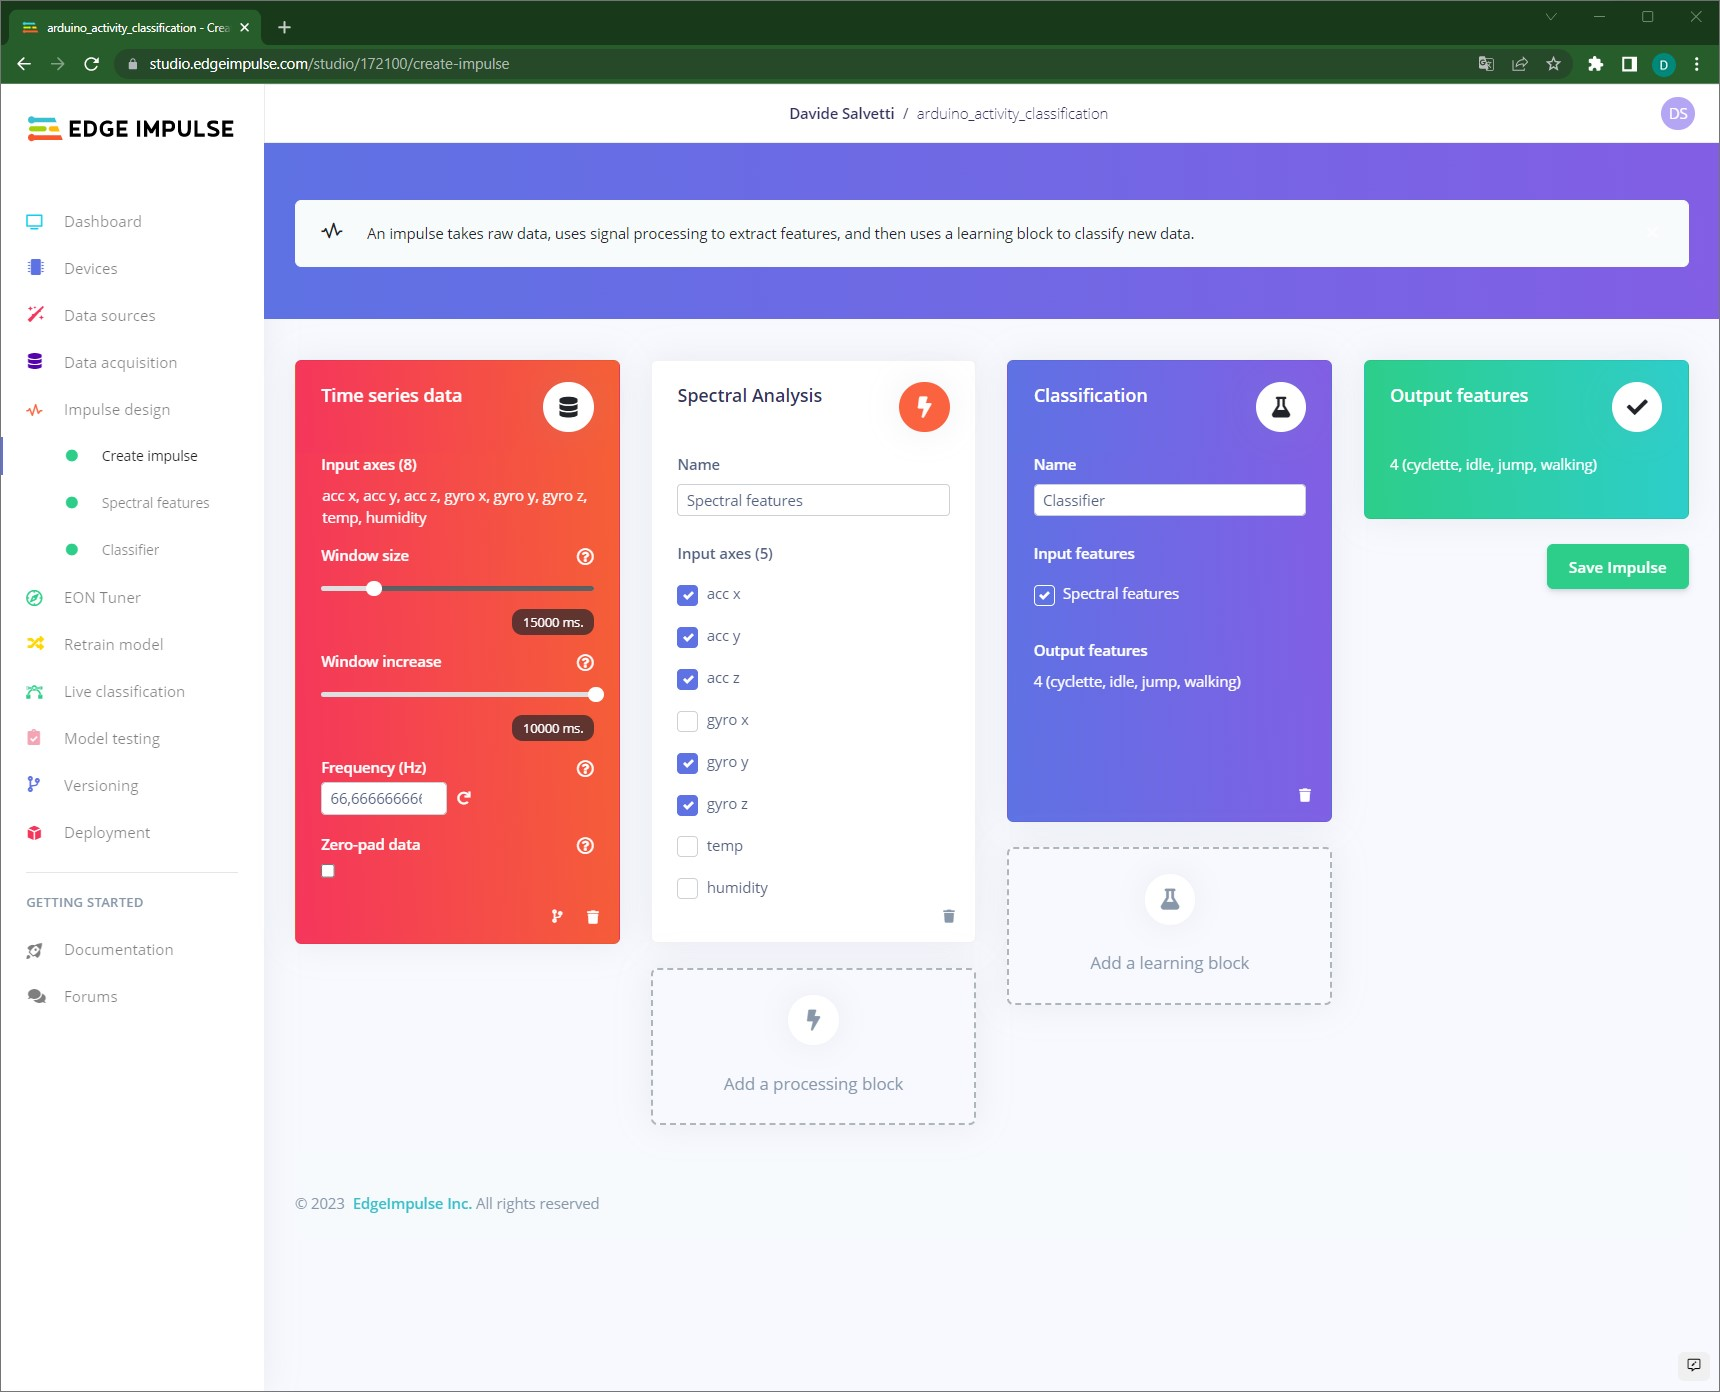
\includegraphics[width=0.5\linewidth]{./ImageFiles/creazione_impulse.jpg}
	\caption{Schermata di Edge Impulse per la creazione di un nuovo \textit{impulse} tramite la scelta di ciascun blocco.}
	\label{fig:creazione_impulse}
\end{figure}
I campioni vengono analizzati su finestre di 15 secondi con una \textit{slinding window} di 10 secondi. La frequenza di campionamento viene ricavata a partire dai dati grazie al campo \texttt{timestamp} ed è pari circa a \SI{66}{\hertz}.
Per il processamento dei dati è stato scelto un DSP che analizza le features spettrali dei segnali provenienti da accelerometro e giroscopio. Come anticipato in precedenza, non sono stati inclusi i campi temperatura e umidità e nemmeno il giroscopio sull'asse x dal momento che non fornisce dati significativi.
Per l'analisi spettrale è stato scelto di introdurre un filtro passa-basso con frequenza di taglio a \SI{20}{\hertz} del sesto ordine ed è stato analizzato il logaritmo della densità spettrale di potenza (figura \ref{fig:spectral_feature}). Una volta definiti i parametri dell'analisi spettrale, il modello estrae le features dai dati di test e viene visualizzato un grafico con i dataset divisi per "somiglianza" delle features; inoltre mostra l'importanza delle features estratte per comparare le diverse classi: alcune delle features più importanti sono il valore quadratico medio dell'accelerometro sull'asse x, la densità spettrale di potenza del giroscopio sull'asse z e la densità spettrale di potenza dell'accelerometro sull'asse y (figura \ref{fig:spectral_feature}).
\begin{figure}[t!]
	\centering
	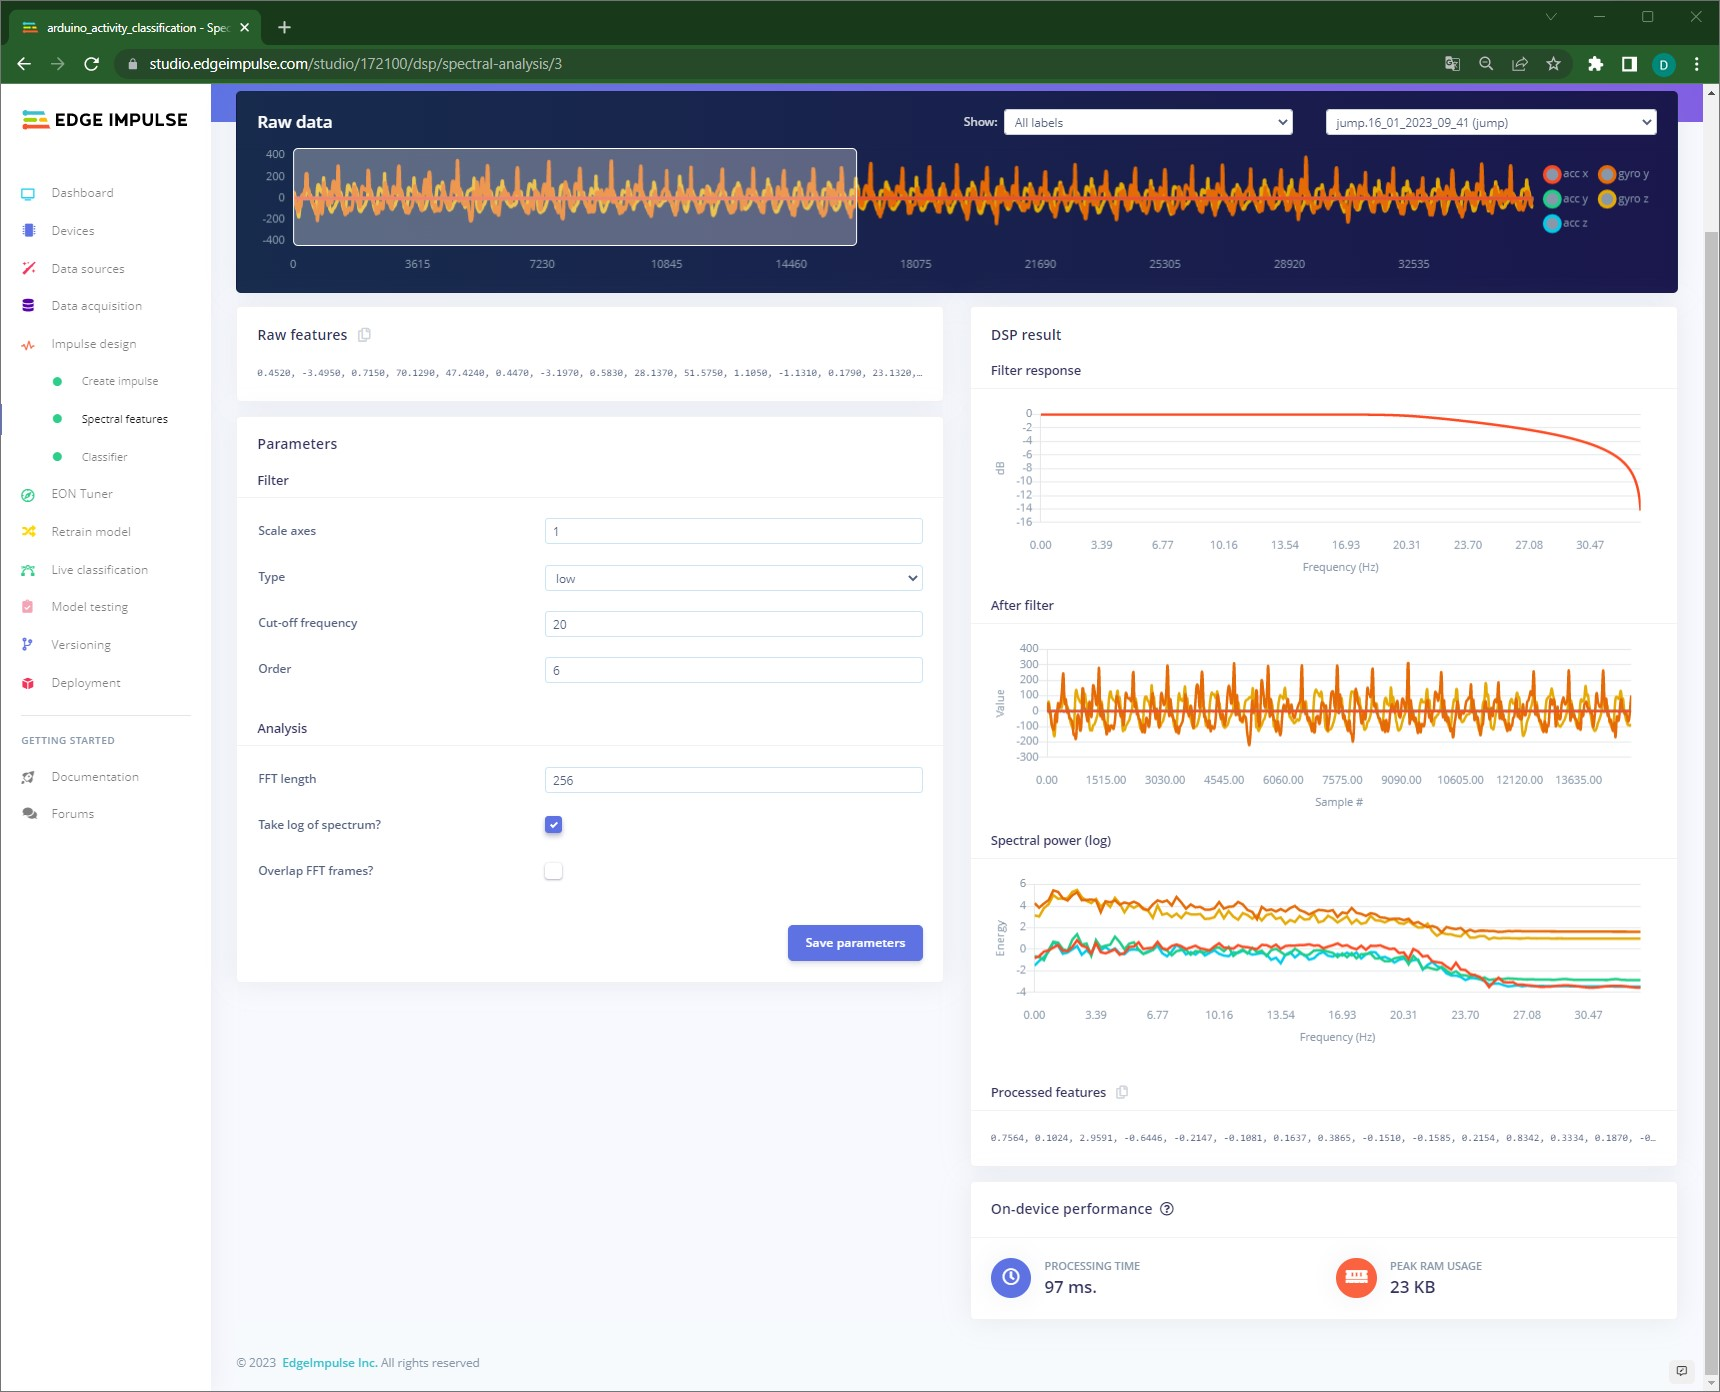
\includegraphics[width=0.49\linewidth]{./ImageFiles/spectral_features.jpg}
	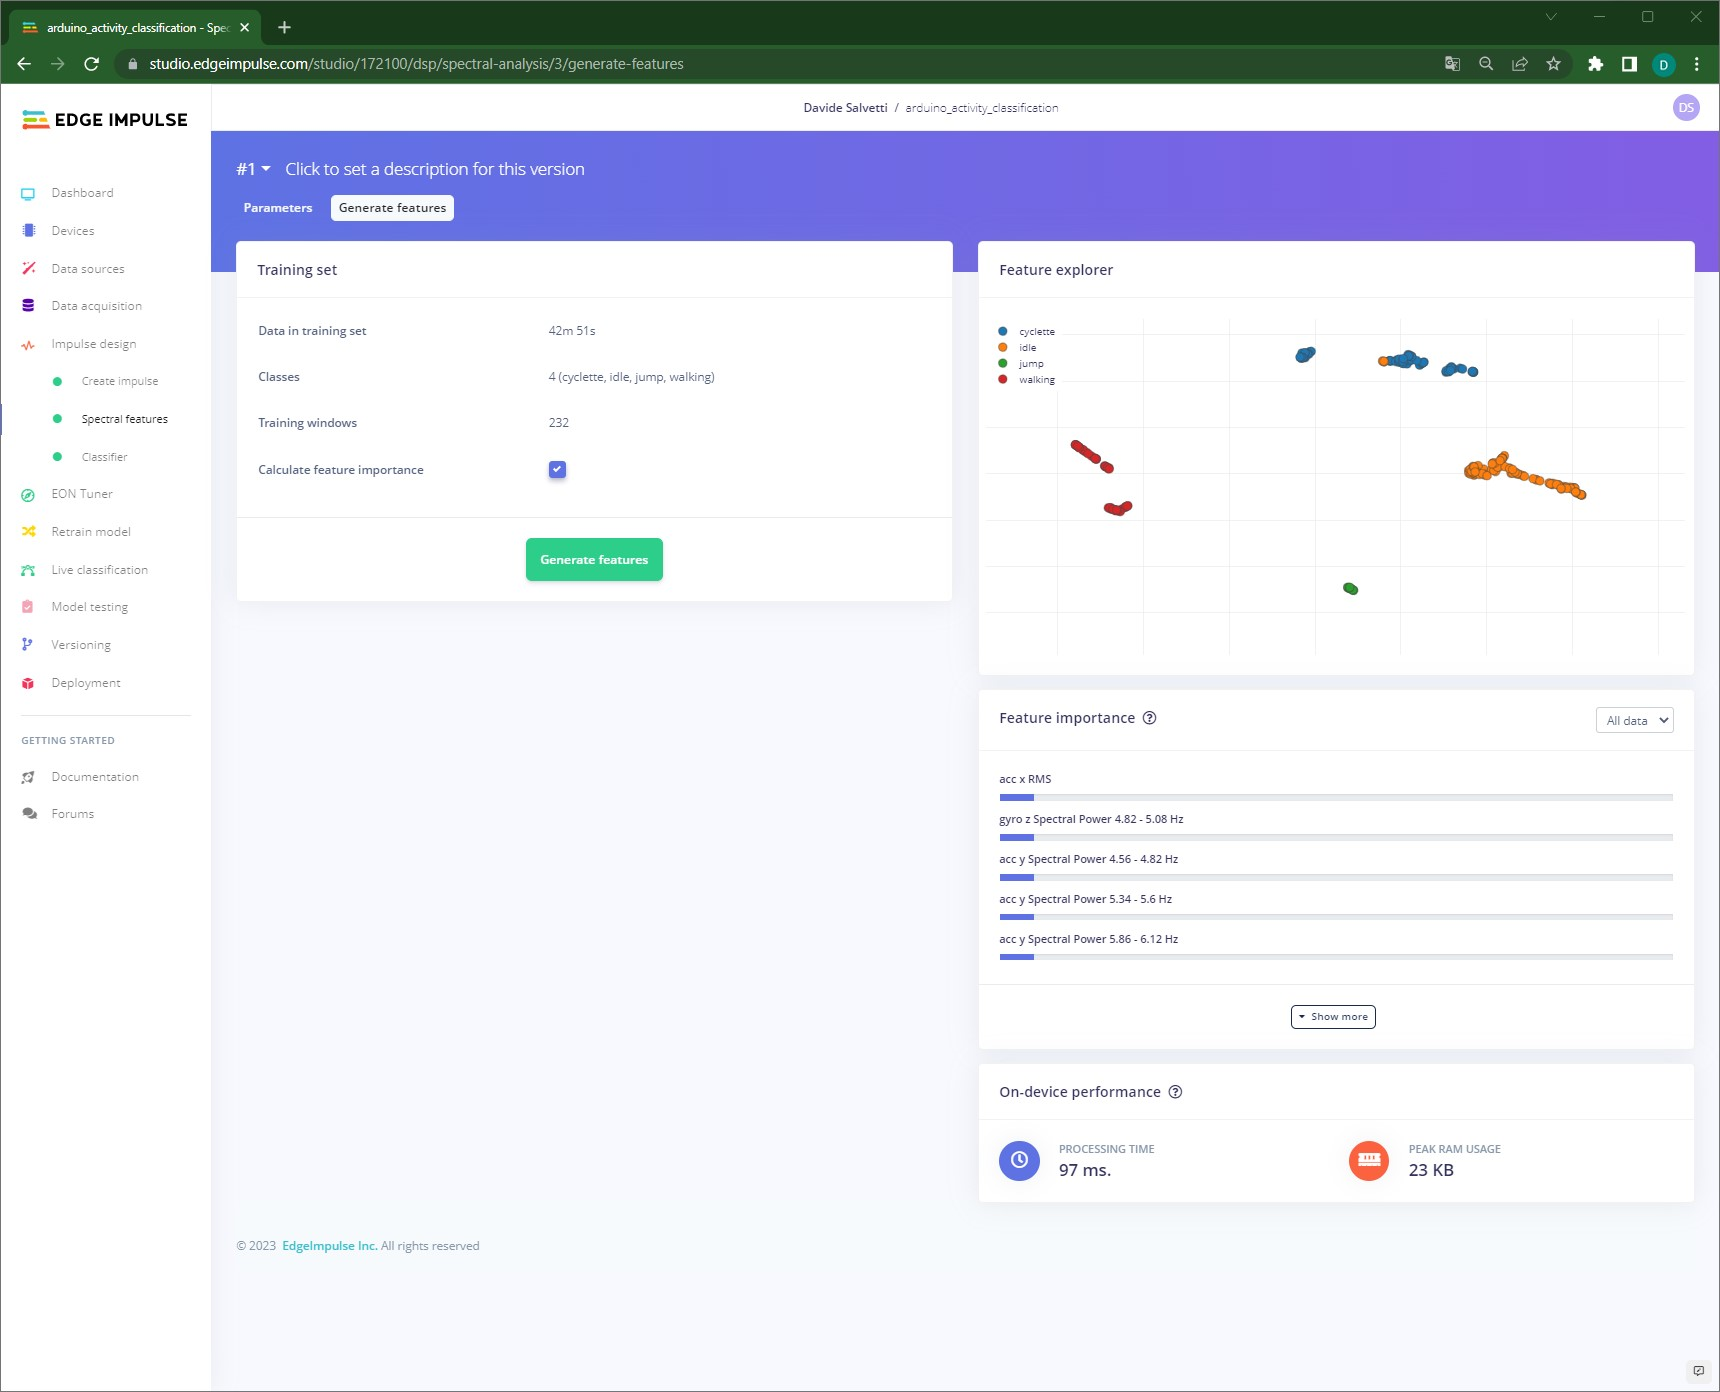
\includegraphics[width=0.49\linewidth]{./ImageFiles/features_extracted.jpg}
	\caption{A sinistra, schermata di Edge Impulse per il settaggio dei parametri per l'estrazione delle features spettrali. A destra, schermata di Edge Impulse per la visualizzazione dell'importanza di ciascuna feature estratta per la distinzione delle varie classi. Inoltre, è possibile osservare le performance stimate sull'Arduino.}
	\label{fig:spectral_feature}
\end{figure}
Come blocco di apprendimento è stato scelto un classificatore. La rete neurale riceve in ingresso 400 features ricavate dal blocco DSP precedente e le analizza tramite due Dense Layer, composti rispettivamente da 32 e 16 neuroni, ed un Output Layer che fornisce in uscita la probabilità di appartenenza delle features in ingresso alle 4 classi. La predizione finale è la classe con probabilità maggiore.
Una volta sviluppato il modello è possibile testarlo sui dati di test (\Fig\ref{fig:model_test}).

\begin{figure}[h!]
	\centering
	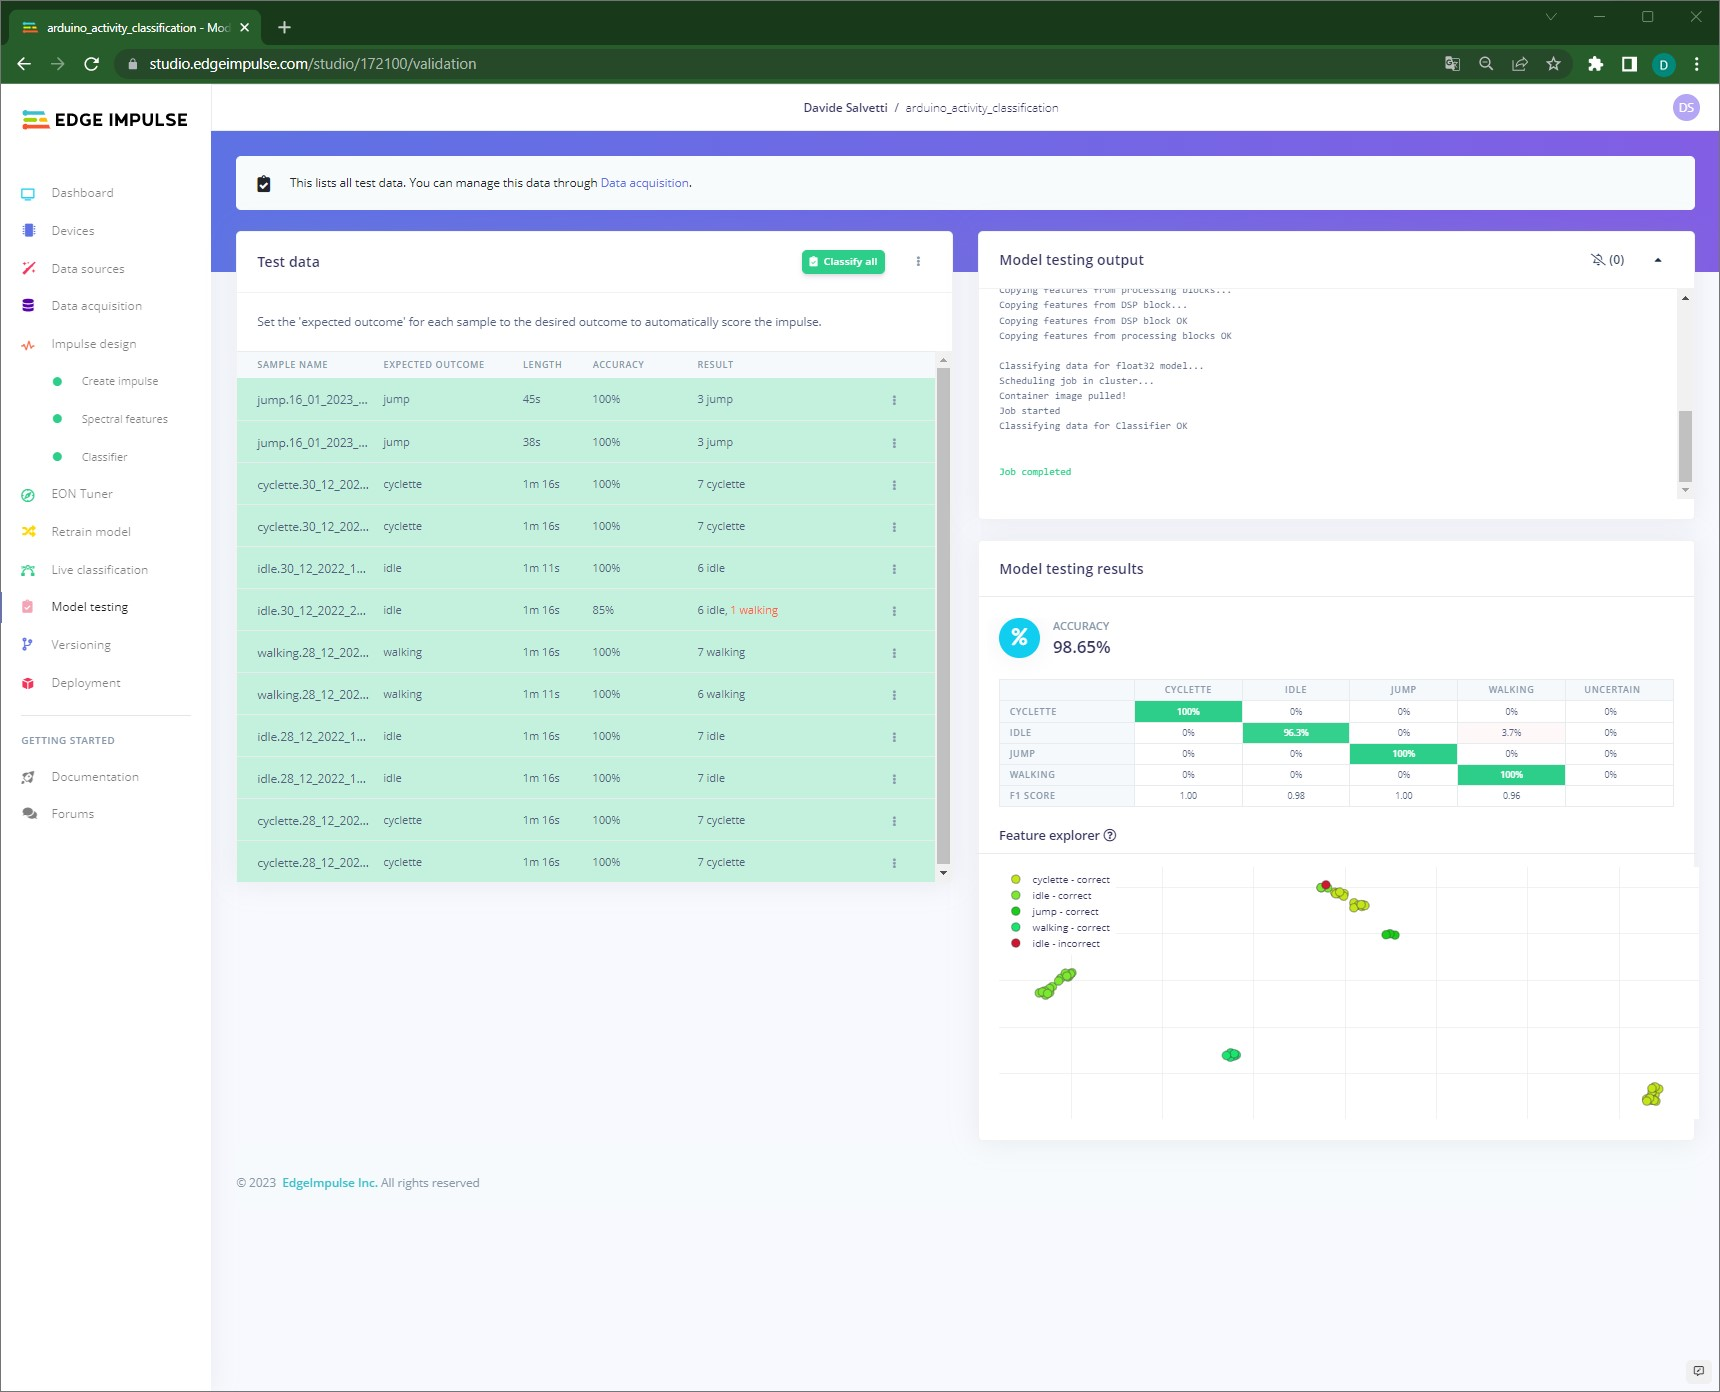
\includegraphics[width=0.5\linewidth]{./ImageFiles/model_test.jpg}
	\caption{Schermata di Edge Impulse per il testing dei dati che mostra l'accuratezza del modello.}
	\label{fig:model_test}
\end{figure}

La fase finale è quella di deploy. Il modello sviluppato, comprensivo del blocco DSP per l'estrazione delle features, può essere scaricato dalla piattaforma Edge Impulse come una libreria di Arduino, la quale può essere caricata direttamente sulla board. 


\subsection{Arduino} \label{arduinoSect}
Il funzionamento base del firmware caricato su Arduino per la classificazione dei dati è mostrato nella figura \ref{fig:SM_classif}.
\begin{figure}[tbh]
	\centering
	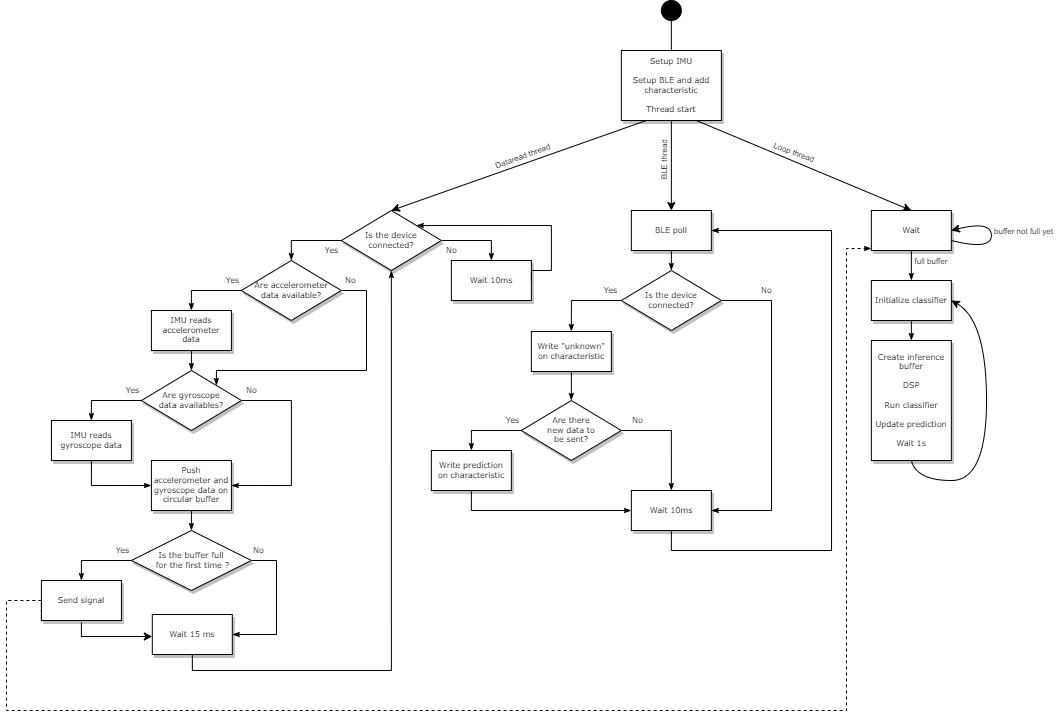
\includegraphics[width=\linewidth]{./ImageFiles/SM_classification}
	\caption{Macchina a stati del firmware di classificazione dei dati sensoriali.}
	\label{fig:SM_classif}
\end{figure}

\noindent
Nel thread \textit{loop}, la chiamata al classificatore corrisponde all'utilizzo delle librerie di Edge Impulse. Questa chiamata richiede come parametri in input il segnale, la variabile in cui salvare la previsione e un parametro che caratterizza l'inferenza. Per quanto riguarda i tempi di classificazione, il tempo necessario per passare da una classificazione alla successiva e quindi per cambiare la previsione è di circa 40-45 secondi. Questo tempo è dovuto al fatto che si deve svuotare il buffer dai dati precedenti e si deve identificare per sei volte la stessa attività prima di definirla come previsione. La previsione viene eseguita ogni 5 secondi e il buffer contiene i dati di \SI{15}{\second} di attività. Per diminuire il tempo necessario per classificare una attività è possibile aumentare la frequenza con cui si esegue l'inferenza.